\documentclass[]{book}
\usepackage{lmodern}
\usepackage{amssymb,amsmath}
\usepackage{ifxetex,ifluatex}
\usepackage{fixltx2e} % provides \textsubscript
\ifnum 0\ifxetex 1\fi\ifluatex 1\fi=0 % if pdftex
  \usepackage[T1]{fontenc}
  \usepackage[utf8]{inputenc}
\else % if luatex or xelatex
  \ifxetex
    \usepackage{mathspec}
  \else
    \usepackage{fontspec}
  \fi
  \defaultfontfeatures{Ligatures=TeX,Scale=MatchLowercase}
\fi
% use upquote if available, for straight quotes in verbatim environments
\IfFileExists{upquote.sty}{\usepackage{upquote}}{}
% use microtype if available
\IfFileExists{microtype.sty}{%
\usepackage{microtype}
\UseMicrotypeSet[protrusion]{basicmath} % disable protrusion for tt fonts
}{}
\usepackage[margin=1in]{geometry}
\usepackage{hyperref}
\hypersetup{unicode=true,
            pdftitle={A Second Semester Statistics Course with R},
            pdfauthor={Mark Greenwood and Katherine Banner},
            pdfborder={0 0 0},
            breaklinks=true}
\urlstyle{same}  % don't use monospace font for urls
\usepackage{natbib}
\bibliographystyle{apalike}
\usepackage{color}
\usepackage{fancyvrb}
\newcommand{\VerbBar}{|}
\newcommand{\VERB}{\Verb[commandchars=\\\{\}]}
\DefineVerbatimEnvironment{Highlighting}{Verbatim}{commandchars=\\\{\}}
% Add ',fontsize=\small' for more characters per line
\usepackage{framed}
\definecolor{shadecolor}{RGB}{248,248,248}
\newenvironment{Shaded}{\begin{snugshade}}{\end{snugshade}}
\newcommand{\KeywordTok}[1]{\textcolor[rgb]{0.13,0.29,0.53}{\textbf{#1}}}
\newcommand{\DataTypeTok}[1]{\textcolor[rgb]{0.13,0.29,0.53}{#1}}
\newcommand{\DecValTok}[1]{\textcolor[rgb]{0.00,0.00,0.81}{#1}}
\newcommand{\BaseNTok}[1]{\textcolor[rgb]{0.00,0.00,0.81}{#1}}
\newcommand{\FloatTok}[1]{\textcolor[rgb]{0.00,0.00,0.81}{#1}}
\newcommand{\ConstantTok}[1]{\textcolor[rgb]{0.00,0.00,0.00}{#1}}
\newcommand{\CharTok}[1]{\textcolor[rgb]{0.31,0.60,0.02}{#1}}
\newcommand{\SpecialCharTok}[1]{\textcolor[rgb]{0.00,0.00,0.00}{#1}}
\newcommand{\StringTok}[1]{\textcolor[rgb]{0.31,0.60,0.02}{#1}}
\newcommand{\VerbatimStringTok}[1]{\textcolor[rgb]{0.31,0.60,0.02}{#1}}
\newcommand{\SpecialStringTok}[1]{\textcolor[rgb]{0.31,0.60,0.02}{#1}}
\newcommand{\ImportTok}[1]{#1}
\newcommand{\CommentTok}[1]{\textcolor[rgb]{0.56,0.35,0.01}{\textit{#1}}}
\newcommand{\DocumentationTok}[1]{\textcolor[rgb]{0.56,0.35,0.01}{\textbf{\textit{#1}}}}
\newcommand{\AnnotationTok}[1]{\textcolor[rgb]{0.56,0.35,0.01}{\textbf{\textit{#1}}}}
\newcommand{\CommentVarTok}[1]{\textcolor[rgb]{0.56,0.35,0.01}{\textbf{\textit{#1}}}}
\newcommand{\OtherTok}[1]{\textcolor[rgb]{0.56,0.35,0.01}{#1}}
\newcommand{\FunctionTok}[1]{\textcolor[rgb]{0.00,0.00,0.00}{#1}}
\newcommand{\VariableTok}[1]{\textcolor[rgb]{0.00,0.00,0.00}{#1}}
\newcommand{\ControlFlowTok}[1]{\textcolor[rgb]{0.13,0.29,0.53}{\textbf{#1}}}
\newcommand{\OperatorTok}[1]{\textcolor[rgb]{0.81,0.36,0.00}{\textbf{#1}}}
\newcommand{\BuiltInTok}[1]{#1}
\newcommand{\ExtensionTok}[1]{#1}
\newcommand{\PreprocessorTok}[1]{\textcolor[rgb]{0.56,0.35,0.01}{\textit{#1}}}
\newcommand{\AttributeTok}[1]{\textcolor[rgb]{0.77,0.63,0.00}{#1}}
\newcommand{\RegionMarkerTok}[1]{#1}
\newcommand{\InformationTok}[1]{\textcolor[rgb]{0.56,0.35,0.01}{\textbf{\textit{#1}}}}
\newcommand{\WarningTok}[1]{\textcolor[rgb]{0.56,0.35,0.01}{\textbf{\textit{#1}}}}
\newcommand{\AlertTok}[1]{\textcolor[rgb]{0.94,0.16,0.16}{#1}}
\newcommand{\ErrorTok}[1]{\textcolor[rgb]{0.64,0.00,0.00}{\textbf{#1}}}
\newcommand{\NormalTok}[1]{#1}
\usepackage{longtable,booktabs}
\usepackage{graphicx,grffile}
\makeatletter
\def\maxwidth{\ifdim\Gin@nat@width>\linewidth\linewidth\else\Gin@nat@width\fi}
\def\maxheight{\ifdim\Gin@nat@height>\textheight\textheight\else\Gin@nat@height\fi}
\makeatother
% Scale images if necessary, so that they will not overflow the page
% margins by default, and it is still possible to overwrite the defaults
% using explicit options in \includegraphics[width, height, ...]{}
\setkeys{Gin}{width=\maxwidth,height=\maxheight,keepaspectratio}
\IfFileExists{parskip.sty}{%
\usepackage{parskip}
}{% else
\setlength{\parindent}{0pt}
\setlength{\parskip}{6pt plus 2pt minus 1pt}
}
\setlength{\emergencystretch}{3em}  % prevent overfull lines
\providecommand{\tightlist}{%
  \setlength{\itemsep}{0pt}\setlength{\parskip}{0pt}}
\setcounter{secnumdepth}{5}
% Redefines (sub)paragraphs to behave more like sections
\ifx\paragraph\undefined\else
\let\oldparagraph\paragraph
\renewcommand{\paragraph}[1]{\oldparagraph{#1}\mbox{}}
\fi
\ifx\subparagraph\undefined\else
\let\oldsubparagraph\subparagraph
\renewcommand{\subparagraph}[1]{\oldsubparagraph{#1}\mbox{}}
\fi

%%% Use protect on footnotes to avoid problems with footnotes in titles
\let\rmarkdownfootnote\footnote%
\def\footnote{\protect\rmarkdownfootnote}

%%% Change title format to be more compact
\usepackage{titling}

% Create subtitle command for use in maketitle
\newcommand{\subtitle}[1]{
  \posttitle{
    \begin{center}\large#1\end{center}
    }
}

\setlength{\droptitle}{-2em}
  \title{A Second Semester Statistics Course with R}
  \pretitle{\vspace{\droptitle}\centering\huge}
  \posttitle{\par}
  \author{Mark Greenwood and Katherine Banner}
  \preauthor{\centering\large\emph}
  \postauthor{\par}
  \predate{\centering\large\emph}
  \postdate{\par}
  \date{2017-07-24}

\usepackage{booktabs}
\usepackage[nottoc,numbib]{tocbibind}
\usepackage{amsmath}
\usepackage{color}
\usepackage{amsbsy}
\usepackage[normalem]{ulem}
\usepackage{cancel}
\usepackage[svgnames]{xcolor}
\usepackage{float}
\usepackage{caption}

\definecolor{purple}{RGB}{76,0,153}

% % make code-output smaller
% \DefineVerbatimEnvironment{Highlighting}{Verbatim}{fontsize=\tiny,commandchars=\\\{\}}
% 

% make console-output smaller:
  \makeatletter
\def\verbatim{\small\@verbatim \frenchspacing\@vobeyspaces \@xverbatim}
\makeatother


%\setlength{\parskip}{0pt}


\setlength{\OuterFrameSep}{-4pt}
\makeatletter
\def\preto{\@verbatim}{\topsep=-10pt \partopsep=-10pt }
\makeatother

\usepackage{amsthm}
\newtheorem{theorem}{Theorem}[chapter]
\newtheorem{lemma}{Lemma}[chapter]
\theoremstyle{definition}
\newtheorem{definition}{Definition}[chapter]
\newtheorem{corollary}{Corollary}[chapter]
\newtheorem{proposition}{Proposition}[chapter]
\theoremstyle{definition}
\newtheorem{example}{Example}[chapter]
\theoremstyle{remark}
\newtheorem*{remark}{Remark}
\begin{document}
\maketitle

{
\setcounter{tocdepth}{1}
\tableofcontents
}
\chapter*{Acknowledgments}\label{acknowledgments}
\addcontentsline{toc}{chapter}{Acknowledgments}

We would like to thank all the students and instructors who have
provided input in the development of the current version of STAT 217 and
that have impacted the choice of topics and how we try to teach them.
Dr.~Robison-Cox initially developed this course using R and much of this
work retains his initial ideas. Many years of teaching these topics and
helping researchers use these topics has helped to refine how they are
presented here. Observing students years after the course has also
helped to refine what we try to teach in the course, trying to prepare
these students for the next levels of statistics courses that they might
encounter and the next class where they might need or want to use
statistics.

I (Greenwood) have intentionally taken a first person perspective at
times to be able to include stories from some of those interactions to
try to help you avoid some of their pitfalls in your current or future
usage of statistics. I would like to thank my wife, Teresa Greenwood,
for allowing me the time and support to work on this. I would also like
to acknowledge Dr.~Gordon Bril (Luther College) who introduced me to
statistics while I was an undergraduate and Dr.~Snehalata Huzurbazar
(University of Wyoming) that guided me to completing my Master's and
Ph.D.~in Statistics and still serves as a valued mentor and friend to
me.

The development of this text was initially supported with funding from
Montana State University's Instructional Innovation Grant Program with a
grant titled Towards more active learning in STAT 217. This book was
born with the goal of having a targeted presentation of topics that we
cover (and few that we don't) that minimizes cost to students and
incorporates the statistical software R from day one and every day after
that. The software is a free, open-source platform and so is dynamically
changing over time. This has necessitated frequent revisions of the
text.

This is Version 3.01 of the book. It fixes a problem created with the
digital links in the book that occurred during Spring 2017. Version 3.0
of the book, prepared for Fall 2016, involved edits, a couple of
partially new sections, and updated R code along with a new format for
how the R code is displayed to more easily distinguish it from other
text. Each revision has involved a similar amount of change with Version
2.0 published in January 2015 and Version 1.0 in January 2014 after
using draft chapters that were initially developed during Fall 2013.

We have made every attempt to keep costs as low as possible by making it
possible for most pages to be printed in black and white. The text (in
full color and with dynamic links) is also available as a free digital
download from Montana State University's ScholarWorks repository at
\url{https://scholarworks.montana.edu/xmlui/handle/1/2999}.

Enjoy your journey from introductory to intermediate statistics!

This work is licensed under the Creative Commons
Attribution-NonCommercial-NoDerivatives 4.0 International License. To
view a copy of this license, visit
\url{http://creativecommons.org/licenses/by-nc-nd/4.0/} or send a letter
to Creative Commons, 444 Castro Street, Suite 900, Mountain View,
California, 94041, USA.

\chapter{Two-Way ANOVA}\label{chapter4}

\section{Situation}\label{section4-1}

In this chapter, we extend the One-Way ANOVA to situations with two
factors or categorical explanatory variables in a method that is
generally called the \textbf{\emph{Two-Way ANOVA}}. This allows
researchers to simultaneously study more than one variable that might
explain variability in the responses and explore whether the impacts of
one variable change depending on the other variable. In some situations,
each observation is so expensive that researchers want to use a single
study to explore two different sets of research questions in the same
round of data collection. For example, a company might want to study
factors that affect the number of defective products per day and are
interested in the impacts of two different types of training programs
and three different levels of production quotas. These methods would
allow engineers to compare the training programs, production quotas, and
see if the training programs work differently for different production
quotas. In a clinical trials context, it is well known that certain
factors can change the performance of certain drugs. For example,
different dosages of a drug might have different benefits or
side-effects on men, versus women or children. \textbf{When the impact
of one factor changes on the level of another factor}, we say that they
\textbf{\emph{interact}}. It is also possible for both factors to be
related to differences in the mean responses and not interact. For
example, suppose there is a difference in the response means between men
and women and a difference among various dosages, but the effect of
increasing the dosage is the same for the male and female subjects. This
is an example of what is called an \textbf{\emph{additive}} type of
model. In general, the world is more complicated than the single factor
models we considered in Chapter \ref{chapter3} can account for,
especially in observational studies, so these models allow us to start
to handle more realistic situations.

Consider the following ``experiment'' where we want to compare the
strength of different brands of paper towels when they are wet. The
response variable will be the time to failure in seconds (a continuous
response variable) when a weight is placed on the towel held at the four
corners. We are interested in studying the differences between brands
and the impact of different amounts of water applied to the towels.

\begin{itemize}
\item
  Predictors (Explanatory Variables): \textbf{A} : \texttt{Brand} (2
  brands of interest, named \emph{B1} and \emph{B2}) and \textbf{B} :
  Number of \texttt{Drops} of water (10, 20, 30 drops).
\item
  Response: \emph{Time} to failure (in seconds) of a towel (\(y\)) with
  a weight sitting in the middle of the towel.
\end{itemize}

\section{Designing a two-way experiment and visualizing
results}\label{section4-2}

Ideally, we want to randomly assign the levels of each factor so that we
can attribute causality to any detected effects and to reduce the
chances of \emph{confounding}. Because there are two factors, we would
need to design a random assignment scheme to select the levels of both
variables. For example, we could randomly select a brand and then
randomly select the number of drops to apply from the levels chosen for
each measurement. Or we could decide on how many observations we want at
each combination of the two factors (ideally having them all equal so
the design is \textbf{\emph{balanced}}) and then randomize the order of
applying the different combinations of levels.

Why might it be important to randomly apply the brand and number of
drops in an experiment? There are situations where the order of
observations can be related to changes in the responses and we want to
be able to eliminate the order of observations from being related to the
levels of the factors. For example, suppose that the area where the
experiment is being performed becomes wet over time and the later
measurements have extra water that gets onto the paper towels and they
tend to fail more quickly. If all the observations for the second brand
were done later in the study, then the \emph{order of observations}
impacts could make the second brand look worse. If the order of
observations is randomized, then even if there is some drift in the
responses over the order of observations it should still be possible to
see the differences in the randomly assigned effects. If the study
incorporates repeated measurements on human subjects, randomizing the
order of treatments they are exposed to can alleviate impacts of them
``learning'' through the study, something that we would not have to
worry about with paper towels.

In observational studies, we do not have the luxury of random
assignment, that is, we cannot randomly assign levels of the treatment
variables to our subjects, so we cannot guarantee that the only
difference between the groups are the explanatory variables. As
discussed before, because we can't control which level of the variables
are assigned to the subjects, we cannot make causal inferences and have
to worry about other variables being the real drivers of the results.
Although we can never establish causal inference with observational
studies, we can generalize our results to a larger population if we have
a representative sample from our population of interest.

It is also possible that we might have studies where some of the
variables are randomly assigned and others are not randomly assignable.
The most common versions of this are what we sometimes call subject
``demographics'', such as sex, income, race, etc. We might be performing
a study where we can randomly assign treatments to these subjects but
might also want to account for differences based on income level, which
we can't assign. In these cases, the scope of inference gets complicated
-- differences seen on randomized variables can be causally interpreted
but you have to be careful to not say that the demographics caused
differences. Suppose that a randomly assigned drug dosage is found to
show differences in male patients but not in female patients. We could
say that the dosage causes differences in males but does not in females.
We are not saying that sex caused the differences but that the causal
differences were modified by the sex of the subjects.

Even when we do have random assignment of treatments it is important to
think about who/what is included in the sample. To get back to the paper
towel example, we are probably interested in more than the sheets of the
rolls we have to work with so if we could randomly select the studied
paper towels from all paper towels made by each brand, our conclusions
could be extended to those populations. That probably would not be
practical, but trying to make sure that the towels are representative of
all made by each brand by checking for defects and maybe picking towels
from a few different rolls would be a good start to being able to extend
inferences beyond the tested towels.

Once random assignment and random sampling is settled, the final aspect
of study design involves deciding on the number of observations that
should be made. The short (glib) answer is to take as many as you can
afford. With more observations comes higher power to detect differences
if they exist, which is a desired attribute of all studies. It is also
important to make sure that you obtain multiple observations at each
combination of the treatment levels, which are called
\textbf{\emph{replicates}}. Having replicate measurements allows
estimation of the mean for each combination of the treatment levels as
well as estimation and testing for an interaction. And we always prefer
having balanced designs because they provide resistance to violation of
some assumptions as noted in Chapter \ref{chapter3}. A
\textbf{\emph{balanced design}} in a Two-Way ANOVA setting involves
having the same sample size for every combination of the levels of the
treatments.

With two categorical explanatory variables, there are now five possible
scenarios for the truth. Different situations are created depending on
whether there is an interaction between the two variables, whether both
variables are important but do not interact, or whether either of the
variables matter at all. Basically, there are five different possible
outcomes in a randomized Two-Way ANOVA study, listed in order of
increasing model complexity:

\begin{enumerate}
\def\labelenumi{\arabic{enumi}.}
\item
  Neither A or B has an effect on the responses (nothing causes
  differences in responses).
\item
  A has an effect, B does not (only A causes differences in responses).
\item
  B has an effect, A does not (only B causes differences in responses).
\item
  Both A and B have effects on response but no interaction (A and B both
  cause differences in responses but the impacts are additive).
\item
  Effect of A differs based on the levels of B, the opposite is also
  true (means for levels of A are different for different levels of B,
  or, simply, A and B interact).
\end{enumerate}

To illustrate these five potential outcomes, we will consider a fake
version of the paper towel example. It ended up being really messy and
complicated to actually perform the experiment as we described it so
these data were simulated to help us understand the Two-Way ANOVA
possibilities in as simple a situation as possible. The first step is to
understand what has been observed (number observations at each
combination of factors) and look at some summary statistics across all
the ``groups''. The data set is available from the course website using:

\begin{Shaded}
\begin{Highlighting}[]
\NormalTok{pt<-}\KeywordTok{read.csv}\NormalTok{(}\StringTok{"http://www.math.montana.edu/courses/s217/documents/pt.csv"}\NormalTok{)}
\NormalTok{pt}\OperatorTok{$}\NormalTok{drops<-}\KeywordTok{factor}\NormalTok{(pt}\OperatorTok{$}\NormalTok{drops)}
\end{Highlighting}
\end{Shaded}

The data set contains five observations per combination of treatment
levels as provided by the \texttt{tally} function. To get counts for
combinations of the variables, use the general formula of
\texttt{tally(x1\textasciitilde{}x2,\ data=...)} although the order of
\texttt{x1} and \texttt{x2} doesn't matter:

\begin{Shaded}
\begin{Highlighting}[]
\KeywordTok{require}\NormalTok{(mosaic)}
\KeywordTok{tally}\NormalTok{(brand }\OperatorTok{~}\StringTok{ }\NormalTok{drops, }\DataTypeTok{data=}\NormalTok{pt)}
\end{Highlighting}
\end{Shaded}

\begin{verbatim}
##      drops
## brand 10 20 30
##    B1  5  5  5
##    B2  5  5  5
\end{verbatim}

The sample sizes in each of the six treatment level combinations of
\texttt{Brand} and \texttt{Drops} {[}(\emph{B1}, 10), (\emph{B1}, 20),
(\emph{B1}, 30), (\emph{B2}, 10), (\emph{B2}, 20), (\emph{B2}, 30){]}
are \(n_{jk} = 5\) for \(j^{th}\) level of \texttt{Brand} (\(j=1, 2\))
and \(k^{th}\) level of \texttt{Drops} (\(k=1, 2, 3\)). The
\texttt{tally} function gives us a \textbf{\emph{contingency table}}
with \(R = 2\) rows (\emph{B1}, \emph{B2}) and \(C = 3\) columns (10,
20, and 30). We'll have more fun with this sort of summary of \(R\) by
\(C\) tables in Chapter \ref{chapter5} -- here it helps us see the
sample size in each combination of factor levels. The \texttt{favstats}
function also helps us dig into the results for all combinations of
factor levels. The notation involves putting both variables after the
``\textasciitilde{}'' with a ``\texttt{+}'' between them. In the output,
the first row contains summary information for the 5 observations for
\texttt{Brand} \emph{B1} and \texttt{Drops} amount 10. It also contains
the sample size in the \texttt{n} column, although here it rolled into a
new set of rows with the standard deviations.

\begin{Shaded}
\begin{Highlighting}[]
\KeywordTok{favstats}\NormalTok{(responses }\OperatorTok{~}\StringTok{ }\NormalTok{brand }\OperatorTok{+}\StringTok{ }\NormalTok{drops, }\DataTypeTok{data=}\NormalTok{pt)}
\end{Highlighting}
\end{Shaded}

\begin{verbatim}
##   brand.drops       min        Q1   median       Q3      max     mean
## 1       B1.10 0.3892621 1.3158737 1.906436 2.050363 2.333138 1.599015
## 2       B2.10 2.3078095 2.8556961 3.001147 3.043846 3.050417 2.851783
## 3       B1.20 0.3838299 0.7737965 1.516424 1.808725 2.105380 1.317631
## 4       B2.20 1.1415868 1.9382142 2.066681 2.838412 3.001200 2.197219
## 5       B1.30 0.2387500 0.9804284 1.226804 1.555707 1.829617 1.166261
## 6       B2.30 0.5470565 1.1205102 1.284117 1.511692 2.106356 1.313946
##          sd n missing
## 1 0.7714970 5       0
## 2 0.3140764 5       0
## 3 0.7191978 5       0
## 4 0.7509989 5       0
## 5 0.6103657 5       0
## 6 0.5686485 5       0
\end{verbatim}

The next step is to visually explore the results across the combinations
of the two explanatory variables. The beanplot can be extended to handle
these sorts of two-way situations only if one of the two variables is a
two-level variable. This is a pretty serious constraint on this display,
so we will show you the plot (Figure \ref{fig:Figure4-1}) but not focus
on the code. The reason beanplots can only handle \(2 \times K\) designs
is that the beans are split along a vertical line for the \(K\) levels
of the other variable. In Figure \ref{fig:Figure4-1}, the \texttt{Brand}
B1 density curves are shaded and the B2 curves are not. In reading these
plots, look for differences in each level and whether those differences
change across the levels of the other variable. Specifically, start with
comparing the two brands for different amounts of water. Do the brands
seem different? Certainly for 10 drops of water the two look different
but not for 30 drops. We can also look for combinations of factors that
produce the highest or lower responses in this display. It appears that
the time to failure is highest in the low water drop groups but as the
water levels increase, the time to failure falls and the differences in
the two brands seem to decrease. The fake data seem to have relatively
similar amounts of variability and distribution shapes -- remembering
that there are only 5 observations available for describing the shape of
responses for each combination. These data were simulated using a normal
distribution and constant variance if that gives you some extra
confidence in assessing these model assumptions.




\begin{Shaded}
\begin{Highlighting}[]
\KeywordTok{require}\NormalTok{(beanplot)}
\KeywordTok{beanplot}\NormalTok{(responses }\OperatorTok{~}\StringTok{ }\NormalTok{brand}\OperatorTok{*}\NormalTok{drops, }\DataTypeTok{data=}\NormalTok{pt, }\DataTypeTok{side=}\StringTok{"b"}\NormalTok{, }\DataTypeTok{col=}\KeywordTok{list}\NormalTok{(}\StringTok{"lightblue"}\NormalTok{,}\StringTok{"white"}\NormalTok{),}
         \DataTypeTok{xlab=}\StringTok{"Drops"}\NormalTok{, }\DataTypeTok{ylab=}\StringTok{"Time"}\NormalTok{, }\DataTypeTok{method=}\StringTok{"jitter"}\NormalTok{,}\DataTypeTok{log=}\StringTok{""}\NormalTok{)}
\KeywordTok{legend}\NormalTok{(}\StringTok{"topright"}\NormalTok{, }\DataTypeTok{bty=}\StringTok{"n"}\NormalTok{, }\KeywordTok{c}\NormalTok{(}\StringTok{"B1"}\NormalTok{,}\StringTok{"B2"}\NormalTok{), }\DataTypeTok{fill=}\KeywordTok{c}\NormalTok{(}\StringTok{"lightblue"}\NormalTok{,}\StringTok{"white"}\NormalTok{))}
\end{Highlighting}
\end{Shaded}

\begin{figure}
\centering
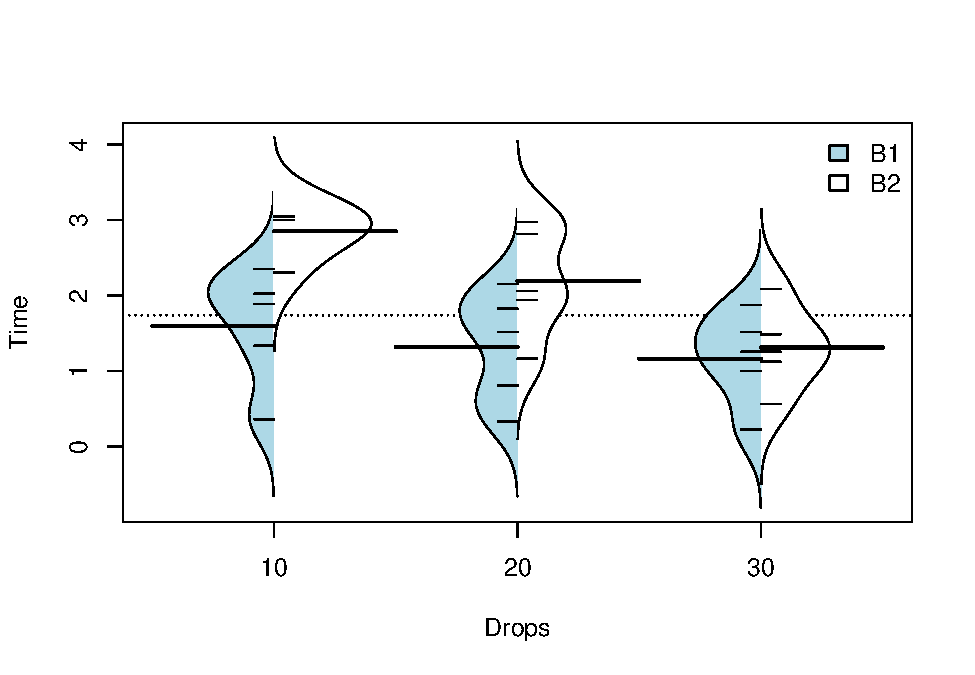
\includegraphics{04-twoWayAnova_files/figure-latex/Figure4-1-1.pdf}
\caption{\label{fig:Figure4-1}Beanplot of paper towel data by \texttt{Drops} (x-axis) and
\texttt{Brand} (side of bean, shaded area for \texttt{Brand} \emph{B1}.}
\end{figure}

The beanplots can't handle situations where both variables have more
than two levels -- we need a simpler display that just focuses on the
means at the combinations of the two explanatory variables. The means
for each combination of levels that you can find in the
\texttt{favstats} output are more usefully used in what is called an
\textbf{\emph{interaction plot}}. Interaction plots display the mean
responses (y-axis) versus levels of one predictor variable on the
x-axis, adding points and lines for each level of the other predictor
variable. Because we don't like any of the available functions in R, we
wrote our own function, called \texttt{intplot} that you can download
using:

\begin{Shaded}
\begin{Highlighting}[]
\KeywordTok{source}\NormalTok{(}\StringTok{"http://www.math.montana.edu/courses/s217/documents/intplot.R"}\NormalTok{)}
\end{Highlighting}
\end{Shaded}

The function allows a formula interface like
\texttt{Y\textasciitilde{}X1*X2} and provides the means \(\pm\) 1 SE
(vertical bars) and adds a legend to help make everything clear.




\begin{figure}
\centering
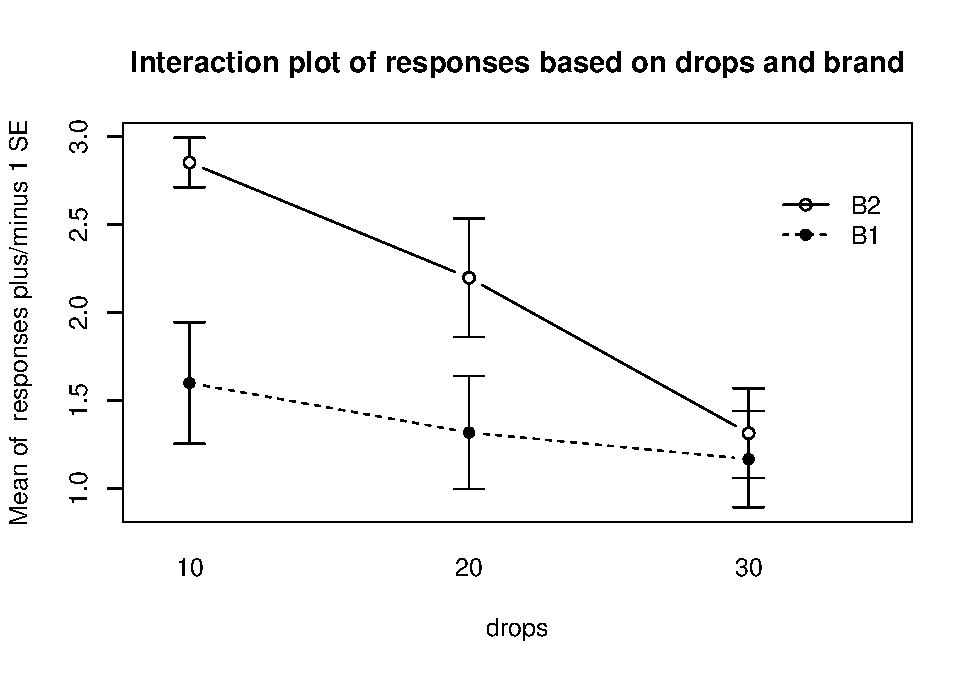
\includegraphics{04-twoWayAnova_files/figure-latex/Figure4-2-1.pdf}
\caption{\label{fig:Figure4-2}Interaction plot of the paper towel data with
\texttt{Drops} on the x-axis.}
\end{figure}

\begin{Shaded}
\begin{Highlighting}[]
\KeywordTok{intplot}\NormalTok{(responses }\OperatorTok{~}\StringTok{ }\NormalTok{brand}\OperatorTok{*}\NormalTok{drops, }\DataTypeTok{data=}\NormalTok{pt)}
\end{Highlighting}
\end{Shaded}

Interaction plots can always be made two different ways by switching the
order of the variables. Figure \ref{fig:Figure4-2} contains
\texttt{Drops} on the x-axis and Figure \ref{fig:Figure4-3} has
\texttt{Brand} on the x-axis. Typically putting the variable with more
levels on the x-axis will make interpretation easier, but not always.
Try both and decide on the one that you like best.




\begin{figure}
\centering
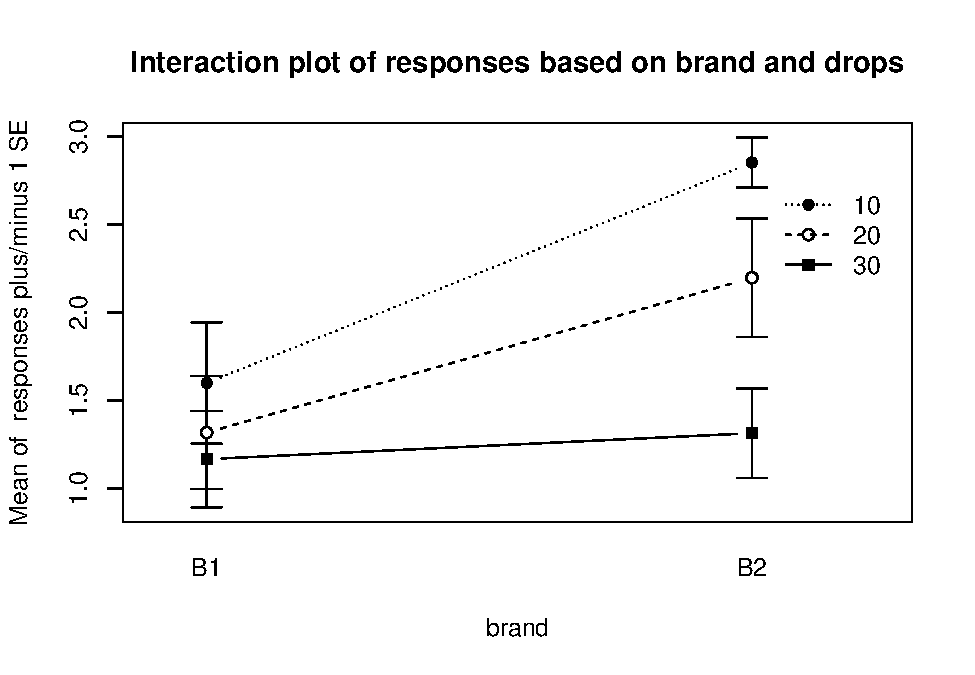
\includegraphics{04-twoWayAnova_files/figure-latex/Figure4-3-1.pdf}
\caption{\label{fig:Figure4-3}Interaction plot of paper towel data with \texttt{Brand} on
the x-axis.}
\end{figure}

\begin{Shaded}
\begin{Highlighting}[]
\KeywordTok{intplot}\NormalTok{(responses }\OperatorTok{~}\StringTok{ }\NormalTok{drops}\OperatorTok{*}\NormalTok{brand, }\DataTypeTok{data=}\NormalTok{pt)}
\end{Highlighting}
\end{Shaded}

The formula in this function builds on our previous notation and now we
include both predictor variables with an ``*" between them. Using an
asterisk between explanatory variables is one way of telling R to
include an interaction between the variables. While the interaction may
or may not be present, the interaction plot helps us to explore those
potential differences.

There are a variety of aspects of the interaction plots to pay attention
to. Initially, the question to answer is whether it appears that there
is an interaction between the predictor variables. When there is an
interaction, you will see \textbf{\emph{non-parallel lines}} in the
interaction plot. You want to look from left to right in the plot and
assess whether the lines are close to parallel, relative to the amount
of variability in the means. If it seems that there is clear visual
evidence of non-parallel lines, then the interaction is likely worth
considering (we will typically use a hypothesis test to formally assess
this -- see discussion below). If the lines look to be close to
parallel, then there probably isn't an interaction between the
variables. Without an interaction present, that means that the
differences across levels of one variable doesn't change based on the
levels of the other variable and vice-versa. This means that we can
consider the \textbf{\emph{main effects}} of each variable on their
own\footnote{We will use ``main effects'' to refer to the two
  explanatory variables in the additive model even if they are not
  randomly assigned to contrast with having those variables interacting
  in the model. It is the one place where we use ``effects'' without
  worrying about random assignment.}. Main effects are much like the
results we found in Chapter \ref{chapter3} where we can compare means
across levels of a single variable except that there are results for two
variables to extract from the model. With the presence of an
interaction, it is complicated to summarize how each variable is
affecting the response variable because their impacts change depending
on the level of the other factor. And plots like the interaction plot
provide us much useful information.

If the lines are not parallel, then focus in on comparing the levels of
one variable as the other variable changes. Remember that the definition
of an interaction is that the differences among levels of one variable
depends on the level of the other variable being considered.
``Visually'' this means comparing the size of the differences in the
lines from left to right. In Figures \ref{fig:Figure4-2} and
\ref{fig:Figure4-3}, the effect of amount of water changes based on the
brand being considered. In Figure \ref{fig:Figure4-3}, the three lines
represent the three water levels. The difference between the brands
(left to right, \emph{B1} to \emph{B2}) is different depending on how
much water was present. It appears that \texttt{Brand} \emph{B2} lasted
longer at the lower water levels but that the difference between the two
brands dropped as the water levels increased. The same story appears in
Figure \ref{fig:Figure4-2}. As the water levels increase (left to right,
10 to 20 to 30 drops), the differences between the two brands decrease.
Of the two versions, Figure \ref{fig:Figure4-2} is probably easier to
read here. The interaction plots also are useful for identifying the
best and worst mean responses for combinations of the treatment levels.
For example, 10 \texttt{Drops} and \texttt{Brand} \emph{B2} lasts
longest, on average, and 30 \texttt{Drops} with \texttt{Brand} \emph{B1}
fails fastest, on average. In this situation, the lines do not appear to
be parallel suggesting that further exploration of the interaction
appears to be warranted.

Before we get to the hypothesis tests to formally make this assessment
(you knew some sort of p-value was coming, right?), we can visualize the
5 different scenarios that could characterize the sorts of results you
could observe in a Two-Way ANOVA situation. Figure \ref{fig:Figure4-4}
shows 4 of the 5 scenarios. In panel (a), when there are no differences
from either variable (Scenario 1), it provides relatively parallel lines
and basically no differences either across \texttt{Drops} levels
(x-axis) or \texttt{Brand} (lines). This would result in no evidence
related to a difference in brands, water levels, or any interaction
between them.




\begin{figure}
\centering
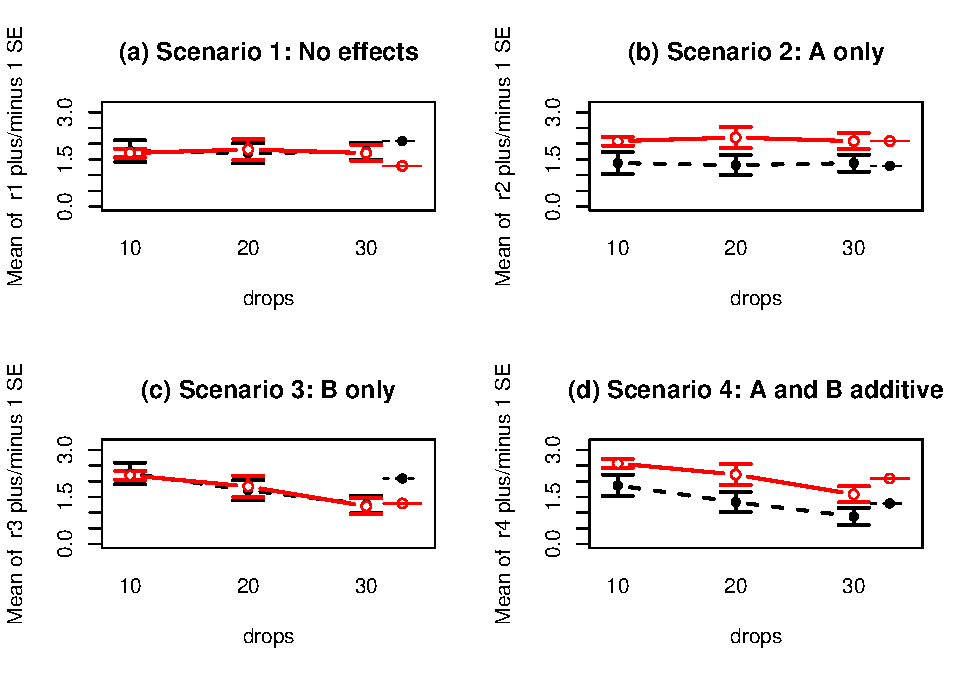
\includegraphics{04-twoWayAnova_files/figure-latex/Figure4-4-1.pdf}
\caption{\label{fig:Figure4-4}Interaction plots of four possible scenarios in the paper
towel study.}
\end{figure}

Scenario 2 (Figure \ref{fig:Figure4-4} panel (b)) incorporates
differences based on factor A (here that is \texttt{Brand}) but no real
difference based on the \texttt{Drops} or any interaction. This results
in a clear shift between the little to no changes in the level of those
lines across water levels. These lines are relatively parallel. We can
see that \texttt{Brand} \emph{B2} is better than \texttt{Brand}
\emph{B1} but that is all we can show with these sorts of results.

Scenario 3 (Figure \ref{fig:Figure4-4} panel (c)) flips the important
variable to B (\texttt{Drops}) and shows decreasing average times as the
water levels increase. Again, the interaction panels show near
parallel-ness in the lines and really just show differences among the
levels of the water. In both Scenarios 2 and 3, we could use a single
variable and drop the other from the model, getting back to a One-Way
ANOVA model, without losing any important information.

Scenario 4 (Figure \ref{fig:Figure4-4} panel (d)) incorporates effects
of A and B, but they are \textbf{\emph{additive}}. That means that the
effect of one variable is the same across the levels of the other
variable. In this experiment, that would mean that \texttt{Drops} has
the same impact on performance regardless of brand and that the brands
differ but each type of difference is the same regardless of levels of
the other variable. The interaction plot lines are more or less parallel
but now the brands are clearly different from each other. The plot shows
the decrease in performance based on increasing water levels and that
\texttt{Brand} \emph{B2} is better than \texttt{Brand} \emph{B1}.
Additive effects show the same difference in lines from left to right in
the interaction plots.

Finally, Scenario 5 (Figure \ref{fig:Figure4-5}) involves an interaction
between the two variables (\texttt{Drops} and \texttt{Brand}). There are
many ways that interactions can present but the main thing is to look
for clearly non-parallel lines. As noted in the previous discussion, the
\texttt{Drops} effect appears to change depending on which level of
\texttt{Brand} is being considered. Note that the plot here described as
Scenario 5 is the same as the initial plot of the results in Figure
\ref{fig:Figure4-2}.




\begin{figure}
\centering
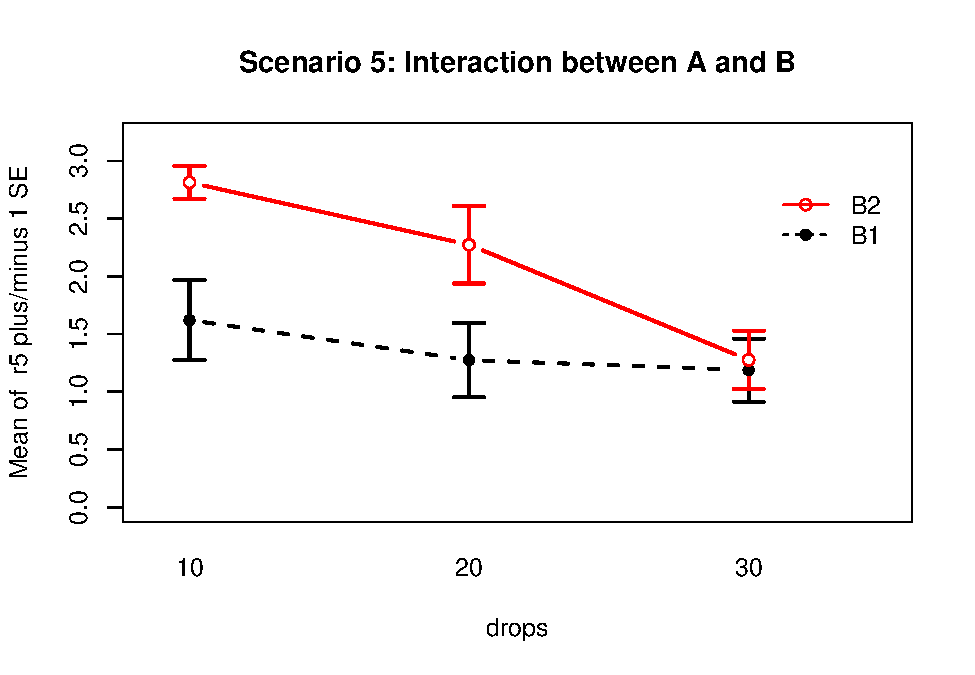
\includegraphics{04-twoWayAnova_files/figure-latex/Figure4-5-1.pdf}
\caption{\label{fig:Figure4-5}Interaction plot of Scenario 5 where it appears that an
interaction is present.}
\end{figure}

The typical modeling protocol is to start with assuming that Scenario 5
is a possible description of the results, related to fitting what is
called the \textbf{\emph{interaction model}}, and then attempt to
simplify the model (to the \textbf{\emph{additive model}}) if warranted.
We need a hypothesis test to help decide if the interaction is ``real''
-- if there is sufficient evidence to prove that there is an
interaction. We need a test because the lines will never be exactly
parallel and, just like in the One-Way ANOVA situation, the amount of
variation around the lines impacts the ability of the model to detect
differences, in this case of an interaction.

\section{Two-Way ANOVA models and hypothesis tests}\label{section4-3}

To assess interactions with two variables, we need to fully describe
models for the additive and interaction scenarios and then develop a
method for assessing evidence of the need for different aspects of the
models. First, we need to define the notation for these models:

\begin{itemize}
\item
  \(y_{ijk}\) is the \(i^{th}\) response from the group for level \(j\)
  of factor A and level \(k\) of factor B

  \begin{itemize}
  \item
    \(j=1,\ldots,J\) ~~~ \(J\) is the number of levels of A
  \item
    \(k=1,\ldots,K\) ~~~ \(K\) is the number of levels of B
  \item
    \(i=1,\ldots,n_{jk}\) ~~~ \(n_{jk}\) is the sample size for level
    \(j\) of factor A and level \(k\) of factor B
  \item
    \(N=\Sigma\Sigma n_{jk}\) is the total sample size (sum of the
    number of observations across all \(JK\) groups)
  \end{itemize}
\end{itemize}

We need to extend our previous discussion of reference-coded models to
develop a Two-Way ANOVA model. We start with the \textbf{\emph{Two-Way
ANOVA interaction model}}:

\[y_{ijk} = \alpha + \tau_j + \gamma_k + \omega_{jk} + \varepsilon_{ijk},\]

where \(\alpha\) is the baseline group mean (for level 1 of A
\textbf{and} level 1 of B), \(\tau_j\) is the deviation for the
\textbf{\emph{main effect}} of A from the baseline for levels
\(2,\ldots,J\), \(\gamma_k\) (gamma \(k\)) is the deviation for the main
effect of B from the baseline for levels \(2,\ldots,K\), and
\(\omega_{jk}\) (omega \(jk\)) is the adjustment for the
\textbf{\emph{interaction effect}} for level \(j\) of factor A and level
\(k\) of factor B for \(j=1,\ldots,J\) and \(k=1,\ldots,K\). In this
model, \(\tau_1\), \(\gamma_1\), and \(\omega_{11}\) are all fixed at 0.
As in Chapter \ref{chapter3}, R will choose the baseline categories
alphabetically but now it is choosing a baseline for both variables and
so our detective work will be doubled to sort this out.

If the interaction term is not important, based on the interaction test
presented below, the \(\omega_{jk}\text{'s}\) can be dropped from the
model and we get a model that corresponds to Scenario 4 above. Scenario
4 is where there are two main effects but no interaction between them.
The \textbf{\emph{additive Two-Way model}} is

\[y_{ijk} = \alpha + \tau_j + \gamma_k + \varepsilon_{ijk},\]

where each component is defined as in the interaction model. The
difference between the interaction and additive models is setting all
the \(\omega_{jk}\text{'s}\) to 0 that are present in the interaction
model. When we set parameters to 0 in models it removes them from the
model. Setting parameters to 0 is how we will develop our hypotheses to
test for an interaction, by testing whether there is evidence enough to
reject that all \(\omega_{jk}\text{'s}=0\).

The interaction test hypotheses are

\begin{itemize}
\item
  \(H_0\): No interaction between A and B in population
  \(\Leftrightarrow\) All \(\omega_{jk}\text{'s}=0\).
\item
  \(H_A\): Interaction between A and B in population \(\Leftrightarrow\)
  At least one \(\omega_{jk}\ne 0\)
\end{itemize}

To perform this test, a new ANOVA \(F\)-test is required (presented
below) but there are also hypotheses relating to the main effects of A
(\(\tau_j\text{'s}\)) and B (\(\gamma_k\text{'s}\)). If evidence is
found to reject the null hypothesis that no interaction is present, then
it is dangerous to ignore it and test for the main effects because
important main effects can be masked by interactions (examples later).
It is important to note that, by definition, \textbf{both variables
matter if an interaction is found to be important} so the main effect
tests may not be very interesting. If the interaction is found to be
important based on the test and retained in the model, you should focus
on the interaction model (also called the \textbf{\emph{full model}}) in
order to understand and describe the form of the interaction among the
variables.

If the interaction test does not return a small p-value, then we have no
evidence to suggest that it is needed and it can be dropped from the
model. In this situation, we would re-fit the model and focus on the
results provided by the additive model -- performing tests for the two
additive main effects. For the first, but not last time, we encounter a
model with more than one variable and test of potential interest. In
models with multiple variables at similar levels (here both are main
effects), we are interested in the results for each variable given that
the other variable is in the model. In many situations, including more
than one variable in a model changes the results for the other variable
even if those variables do not interact. The reason for this is more
clear in Chapter \ref{chapter8} and really only matters here if we have
unbalanced designs, but we need to start adding a short modifier to our
discussions of main effects -- they are the results \emph{conditional
on} or \emph{adjusting for} or, simply, \emph{given}, the other
variable(s) in the model. Specifically, the hypotheses for the two main
effects are:

\begin{itemize}
\item
  Main effect test for A:

  \begin{itemize}
  \item
    \(H_0\): No differences in means across levels of A in population,
    given B in the model \(\Leftrightarrow\) All \(\tau_j\text{'s} = 0\)
    in additive model.
  \item
    \(H_A\): Some difference in means across levels A in population,
    given B in the model \(\Leftrightarrow\) At least one
    \(\tau_j \ne 0\), in additive model.
  \end{itemize}
\item
  Main effect test for B:

  \begin{itemize}
  \item
    \(H_0\): No differences in means across levels of B in population,
    given A in the model \(\Leftrightarrow\) All
    \(\gamma_k\text{'s} = 0\) in additive model.
  \item
    \(H_A\): Some difference in means across levels B in population,
    given A in the model \(\Leftrightarrow\) At least one
    \(\gamma_k \ne 0\), in additive model.
  \end{itemize}
\end{itemize}

In order to test these effects (interaction in the interaction model and
main effects in the additive model), \(F\)-tests are developed using
Sums of Squares, Mean Squares, and degrees of freedom similar to those
in Chapter \ref{chapter3}. We won't worry about the details of the sums
of squares formulas but you should remember the sums of squares
decomposition, which still applies\footnote{In the standard ANOVA table,
  \(\text{SS}_A + \text{SS}_B + \text{SS}_{AB} + \text{SS}_E = \text{SS}_{\text{Total}}\).
  However, to get the tests we really desire when our designs are not
  balanced, a slight modification of the SS is used, using what are
  called Type II sums of squares and this result doesn't hold in the
  output you will see for additive models. This is discussed further
  below.}. Table \ref{tab:Table4-1} summarizes the ANOVA results you
will obtain for the interaction model and Table \ref{tab:Table4-2}
provides the similar general results for the additive model. As we saw
in Chapter \ref{chapter3}, the degrees of freedom are the amount of
information that is free to vary at a particular level and that rule
generally holds here. For example, for factor A with \(J\) levels, there
are \(J-1\) parameters that are free since the baseline is fixed. The
residual degrees of freedom for both models are not as easily explained
but have simple formula. Note that the sum of the degrees of freedom
from the main effects, (interaction if present), and error need to equal
\(N-1\), just like in the One-Way ANOVA table.



\begin{longtable}[]{@{}lllll@{}}
\caption{\label{tab:Table4-1} Interaction Model ANOVA Table.}\tabularnewline
\toprule
\begin{minipage}[b]{0.16\columnwidth}\raggedright\strut
\textbf{Source}~~~~\strut
\end{minipage} & \begin{minipage}[b]{0.17\columnwidth}\raggedright\strut
\textbf{DF}~~~~~\strut
\end{minipage} & \begin{minipage}[b]{0.19\columnwidth}\raggedright\strut
\textbf{SS}\strut
\end{minipage} & \begin{minipage}[b]{0.21\columnwidth}\raggedright\strut
\textbf{MS}\strut
\end{minipage} & \begin{minipage}[b]{0.12\columnwidth}\raggedright\strut
\textbf{F-statistics}\strut
\end{minipage}\tabularnewline
\midrule
\endfirsthead
\toprule
\begin{minipage}[b]{0.16\columnwidth}\raggedright\strut
\textbf{Source}~~~~\strut
\end{minipage} & \begin{minipage}[b]{0.17\columnwidth}\raggedright\strut
\textbf{DF}~~~~~\strut
\end{minipage} & \begin{minipage}[b]{0.19\columnwidth}\raggedright\strut
\textbf{SS}\strut
\end{minipage} & \begin{minipage}[b]{0.21\columnwidth}\raggedright\strut
\textbf{MS}\strut
\end{minipage} & \begin{minipage}[b]{0.12\columnwidth}\raggedright\strut
\textbf{F-statistics}\strut
\end{minipage}\tabularnewline
\midrule
\endhead
\begin{minipage}[t]{0.16\columnwidth}\raggedright\strut
A\strut
\end{minipage} & \begin{minipage}[t]{0.17\columnwidth}\raggedright\strut
\(J-1\)\strut
\end{minipage} & \begin{minipage}[t]{0.19\columnwidth}\raggedright\strut
\(\text{SS}_A\)\strut
\end{minipage} & \begin{minipage}[t]{0.21\columnwidth}\raggedright\strut
\(\text{MS}_A=\text{SS}_A/\text{df}_A\)\strut
\end{minipage} & \begin{minipage}[t]{0.12\columnwidth}\raggedright\strut
\(\text{MS}_A/\text{MS}_E\)\strut
\end{minipage}\tabularnewline
\begin{minipage}[t]{0.16\columnwidth}\raggedright\strut
B\strut
\end{minipage} & \begin{minipage}[t]{0.17\columnwidth}\raggedright\strut
\(K-1\)\strut
\end{minipage} & \begin{minipage}[t]{0.19\columnwidth}\raggedright\strut
\(\text{SS}_B\)\strut
\end{minipage} & \begin{minipage}[t]{0.21\columnwidth}\raggedright\strut
\(\text{MS}_B=\text{SS}_B/\text{df}_B\)\strut
\end{minipage} & \begin{minipage}[t]{0.12\columnwidth}\raggedright\strut
\(\text{MS}_B/\text{MS}_E\)\strut
\end{minipage}\tabularnewline
\begin{minipage}[t]{0.16\columnwidth}\raggedright\strut
A:B (interaction)\strut
\end{minipage} & \begin{minipage}[t]{0.17\columnwidth}\raggedright\strut
\((J-1)(K-1)\)\strut
\end{minipage} & \begin{minipage}[t]{0.19\columnwidth}\raggedright\strut
\(\text{SS}_{AB}\)\strut
\end{minipage} & \begin{minipage}[t]{0.21\columnwidth}\raggedright\strut
\(\text{MS}_{AB}=\text{SS}_{AB}/\text{df}_{AB}\)\strut
\end{minipage} & \begin{minipage}[t]{0.12\columnwidth}\raggedright\strut
\(\text{MS}_{AB}/\text{MS}_E\)\strut
\end{minipage}\tabularnewline
\begin{minipage}[t]{0.16\columnwidth}\raggedright\strut
Error\strut
\end{minipage} & \begin{minipage}[t]{0.17\columnwidth}\raggedright\strut
\(N-J-K+1\)\strut
\end{minipage} & \begin{minipage}[t]{0.19\columnwidth}\raggedright\strut
\(\text{SS}_E\)\strut
\end{minipage} & \begin{minipage}[t]{0.21\columnwidth}\raggedright\strut
\(\text{MS}_E=\text{SS}_E/\text{df}_E\)\strut
\end{minipage} & \begin{minipage}[t]{0.12\columnwidth}\raggedright\strut
\strut
\end{minipage}\tabularnewline
\begin{minipage}[t]{0.16\columnwidth}\raggedright\strut
\textcolor{red}{\textbf{Total}}\strut
\end{minipage} & \begin{minipage}[t]{0.17\columnwidth}\raggedright\strut
\(\color{red}{\mathbf{N-1}}\)\strut
\end{minipage} & \begin{minipage}[t]{0.19\columnwidth}\raggedright\strut
\(\color{red}{\textbf{SS}_{\textbf{Total}}}\)\strut
\end{minipage} & \begin{minipage}[t]{0.21\columnwidth}\raggedright\strut
\strut
\end{minipage} & \begin{minipage}[t]{0.12\columnwidth}\raggedright\strut
\strut
\end{minipage}\tabularnewline
\bottomrule
\end{longtable}



\begin{longtable}[]{@{}lllll@{}}
\caption{\label{tab:Table4-2} Additive Model ANOVA Table.}\tabularnewline
\toprule
\begin{minipage}[b]{0.17\columnwidth}\raggedright\strut
\textbf{Source}~~~~\strut
\end{minipage} & \begin{minipage}[b]{0.18\columnwidth}\raggedright\strut
\textbf{DF}~~~~~\strut
\end{minipage} & \begin{minipage}[b]{0.21\columnwidth}\raggedright\strut
\textbf{SS}\strut
\end{minipage} & \begin{minipage}[b]{0.18\columnwidth}\raggedright\strut
\textbf{MS}\strut
\end{minipage} & \begin{minipage}[b]{0.12\columnwidth}\raggedright\strut
\textbf{F-statistics}\strut
\end{minipage}\tabularnewline
\midrule
\endfirsthead
\toprule
\begin{minipage}[b]{0.17\columnwidth}\raggedright\strut
\textbf{Source}~~~~\strut
\end{minipage} & \begin{minipage}[b]{0.18\columnwidth}\raggedright\strut
\textbf{DF}~~~~~\strut
\end{minipage} & \begin{minipage}[b]{0.21\columnwidth}\raggedright\strut
\textbf{SS}\strut
\end{minipage} & \begin{minipage}[b]{0.18\columnwidth}\raggedright\strut
\textbf{MS}\strut
\end{minipage} & \begin{minipage}[b]{0.12\columnwidth}\raggedright\strut
\textbf{F-statistics}\strut
\end{minipage}\tabularnewline
\midrule
\endhead
\begin{minipage}[t]{0.17\columnwidth}\raggedright\strut
A\strut
\end{minipage} & \begin{minipage}[t]{0.18\columnwidth}\raggedright\strut
\(J-1\)\strut
\end{minipage} & \begin{minipage}[t]{0.21\columnwidth}\raggedright\strut
\(\text{SS}_A\)\strut
\end{minipage} & \begin{minipage}[t]{0.18\columnwidth}\raggedright\strut
\(\text{MS}_A=\text{SS}_A/\text{df}_A\)\strut
\end{minipage} & \begin{minipage}[t]{0.12\columnwidth}\raggedright\strut
\(\text{MS}_A/\text{MS}_E\)\strut
\end{minipage}\tabularnewline
\begin{minipage}[t]{0.17\columnwidth}\raggedright\strut
B\strut
\end{minipage} & \begin{minipage}[t]{0.18\columnwidth}\raggedright\strut
\(K-1\)\strut
\end{minipage} & \begin{minipage}[t]{0.21\columnwidth}\raggedright\strut
\(\text{SS}_B\)\strut
\end{minipage} & \begin{minipage}[t]{0.18\columnwidth}\raggedright\strut
\(\text{MS}_B=\text{SS}_B/\text{df}_B\)\strut
\end{minipage} & \begin{minipage}[t]{0.12\columnwidth}\raggedright\strut
\(\text{MS}_B/\text{MS}_E\)\strut
\end{minipage}\tabularnewline
\begin{minipage}[t]{0.17\columnwidth}\raggedright\strut
Error\strut
\end{minipage} & \begin{minipage}[t]{0.18\columnwidth}\raggedright\strut
\(N-J-K+1\)\strut
\end{minipage} & \begin{minipage}[t]{0.21\columnwidth}\raggedright\strut
\(\text{SS}_E\)\strut
\end{minipage} & \begin{minipage}[t]{0.18\columnwidth}\raggedright\strut
\(\text{MS}_E=\text{SS}_E/\text{df}_E\)\strut
\end{minipage} & \begin{minipage}[t]{0.12\columnwidth}\raggedright\strut
\strut
\end{minipage}\tabularnewline
\begin{minipage}[t]{0.17\columnwidth}\raggedright\strut
\textcolor{red}{\textbf{Total}}\strut
\end{minipage} & \begin{minipage}[t]{0.18\columnwidth}\raggedright\strut
\(\color{red}{\mathbf{N-1}}\)\strut
\end{minipage} & \begin{minipage}[t]{0.21\columnwidth}\raggedright\strut
\(\color{red}{\textbf{SS}_{\textbf{Total}}}\)\strut
\end{minipage} & \begin{minipage}[t]{0.18\columnwidth}\raggedright\strut
\strut
\end{minipage} & \begin{minipage}[t]{0.12\columnwidth}\raggedright\strut
\strut
\end{minipage}\tabularnewline
\bottomrule
\end{longtable}

The mean squares are formed by taking the sums of squares (we'll let R
find those for us) and dividing by the \(df\) in the row. The
\(F\)-ratios are found by taking the mean squares from the row and
dividing by the mean squared error (\(\text{MS}_E\)). They follow
\(F\)-distributions with numerator degrees of freedom from the row and
denominator degrees of freedom from the Error row (in R output this the
\texttt{Residuals} row). It is possible to develop permutation tests for
these methods but some technical issues arise in doing permutation tests
for interaction model components so we will not use them here. This
means we will have to place even more emphasis on meeting the
assumptions since we only have the parametric method available.

With some basic expectations about the ANOVA tables and \(F\)-statistic
construction in mind, we can get to actually estimating the models and
exploring the results. The first example involves the fake paper towel
data displayed in Figure \ref{fig:Figure4-1} and \ref{fig:Figure4-2}. It
appeared that Scenario 5 was the correct story since the lines were not
parallel, but we need to know whether there is evidence to suggest that
the interaction is ``real'' and we get that through the interaction
hypothesis test. To fit the interaction model using \texttt{lm}, the
general formulation is
\texttt{lm(y\ \textasciitilde{}\ x1*x2,\ data=...)}. The order of the
variables doesn't matter and the most important part of the model, to
start with, relates to the interaction of the variables.

The ANOVA table output shows the results for the interaction model
obtained by running the \texttt{anova} function on the model called
\texttt{m1}. Specifically, the test that
\(H_0: \text{ All } \omega_{jk}\text{'s} = 0\) has a test statistic of
\(F(2,24)=1.92\) (in bold in the output from the row with brands:drops)
and a p-value of 0.17. So there is insufficient evidence to reject the
null hypothesis of no interaction, with a 17\% chance we would observe a
difference in the \(\omega_{jk}\text{'s}\) like we did or more extreme
if the \(\omega_{jk}\text{'s}\) really were all 0. For the interaction
model components, R presents them with a colon, \texttt{:}, between the
variable names.

\begin{Shaded}
\begin{Highlighting}[]
\NormalTok{m1<-}\KeywordTok{lm}\NormalTok{(responses }\OperatorTok{~}\StringTok{ }\NormalTok{brand}\OperatorTok{*}\NormalTok{drops, }\DataTypeTok{data=}\NormalTok{pt)}
\KeywordTok{anova}\NormalTok{(m1)}
\end{Highlighting}
\end{Shaded}

\begin{verbatim}
## Analysis of Variance Table
## 
## Response: responses
##             Df Sum Sq Mean Sq F value   Pr(>F)
## brand        1 4.3322  4.3322 10.5192 0.003458
## drops        2 4.8581  2.4290  5.8981 0.008251
## brand:drops  2 1.5801  0.7901  1.9184 0.168695
## Residuals   24 9.8840  0.4118
\end{verbatim}

It is useful to display the estimates from this model and we can utilize
\texttt{plot(allEffects(modelname))} to visualize the results for the
terms in our models. If we turn on the options for \texttt{grid=T},
\texttt{multiline=T}, and \texttt{ci.\ style="bars"} we will get a more
useful version of the basic ``effect plot'' for Two-Way ANOVA models
with interaction. The results of the estimated interaction model are
displayed in Figure \ref{fig:Figure4-6}, which looks very similar to our
previous interaction plot. The only difference is that this comes from
model that assumes equal variance and these plots show 95\% confidence
intervals for the means instead of the 1 standard error used above.



\begin{figure}
\centering
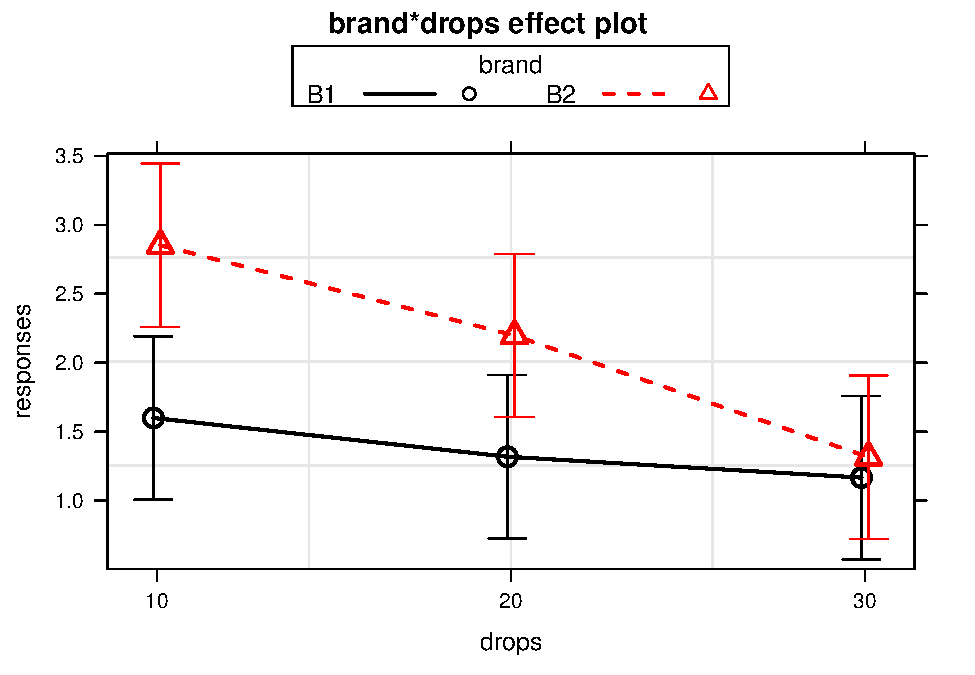
\includegraphics{04-twoWayAnova_files/figure-latex/Figure4-6-1.pdf}
\caption{\label{fig:Figure4-6}Plot of estimated results of interaction model.}
\end{figure}

In the absence of evidence to include the interaction, the model should
be simplified to the additive model and the interpretation focused on
each main effect, conditional on having the other variable in the model.
To fit an additive model and not include an interaction, the model
formula involves a ``+'' instead of a ``*" between the explanatory
variables.

\begin{Shaded}
\begin{Highlighting}[]
\NormalTok{m2<-}\KeywordTok{lm}\NormalTok{(responses }\OperatorTok{~}\StringTok{ }\NormalTok{brand }\OperatorTok{+}\StringTok{ }\NormalTok{drops, }\DataTypeTok{data=}\NormalTok{pt)}
\KeywordTok{anova}\NormalTok{(m2)}
\end{Highlighting}
\end{Shaded}

\begin{verbatim}
## Analysis of Variance Table
## 
## Response: responses
##           Df  Sum Sq Mean Sq F value   Pr(>F)
## brand      1  4.3322  4.3322  9.8251 0.004236
## drops      2  4.8581  2.4290  5.5089 0.010123
## Residuals 26 11.4641  0.4409
\end{verbatim}

The p-values for the main effects of \texttt{brand} and \texttt{drops}
change slightly from the results in the interaction model due to changes
in the \(\text{MS}_E\) from 0.4118 to 0.4409 (more variability is left
over in the simpler model) and the \(\text{DF}_{\text{error}}\) that
increases from 24 to 26. In both models, the
\(\text{SS}_{\text{Total}}\) is the same (20.6544). In the interaction
model,

\[\begin{array}{rl}
\text{SS}_{\text{Total}} & = \text{SS}_{\text{brand}} + \text{SS}_{\text{drops}}
+ \text{SS}_{\text{brand:drops}} + \text{SS}_{\text{E}}\\
& = 4.3322 + 4.8581 + 1.5801 + 9.8840\\
& = 20.6544\\
\end{array}\]

In the additive model, the variability that was attributed to the
interaction term in the interaction model
(\(\text{SS}_{\text{brand:drops}} = 1.5801\)) is pushed into the
\(\text{SS}_{\text{E}}\), which increases from 9.884 to 11.4641. The
sums of squares decomposition in the additive model is

\[\begin{array}{rl}
\text{SS}_{\text{Total}} & = \text{SS}_{\text{brand}} + \text{SS}_{\text{drops}}
 + \text{SS}_{\text{E}} \\
& = 4.3322 + 4.8581 + 11.4641 \\
& = 20.6544 \\
\end{array}\]

This shows that the sums of squares decomposition applies in these more
complicated models as it did in the One-Way ANOVA. It also shows that if
the interaction is removed from the model, that variability is lumped in
with the other unexplained variability that goes in the
\(\text{SS}_{\text{E}}\) in any model.

The fact that the sums of squares decomposition can be applied here is
useful, except that there is a small issue with the main effect tests in
the ANOVA table results that follow this decomposition when the design
is not balanced. It ends up that the tests in a typical ANOVA table are
only conditional on the tests higher up in the table. For example, in
the additive model ANOVA table, the \texttt{Brand} test is not
conditional on the \texttt{Drops} effect, but the \texttt{Drops} effect
is conditional on the \texttt{Brand} effect. To fix this issue, we have
to use another type of sums of squares, called \textbf{\emph{Type II
sums of squares}}. They will no longer always follow the rules of the
sums of squares decomposition but they will test the desired hypotheses.
Specifically, they provide each test conditional on any other terms at
the same level of the model and match the hypotheses written out earlier
in this section. To get the ``correct'' ANOVA results, the \texttt{car}
(\citet{R-car}, \citet{Fox2011}) package is required. We use the
\texttt{Anova} function on our linear models from here forward to get
the ``right'' tests in our ANOVA tables. Note how the case-sensitive
nature of R code shows up in the use of the capital-A \texttt{Anova}
function instead of the \texttt{anova} function used previously. In this
case, because the design was balanced, the results are the same using
either function. Observational studies rarely generate balanced designs
(some designed studies can result in unbalanced designs) so we will
generally just use the Type II version of the sums of squares. The
\texttt{Anova} results using the Type II sums of squares are slightly
more conservative than the results from \texttt{anova}, which are called
Type I sums of squares. The sums of squares decomposition no longer can
be applied, but it is a small sacrifice to get each test after adjusting
for all other variables\footnote{Actually, the tests are only
  conditional on other main effects if Type II Sums of Squares are used
  for an interaction model.}.

\begin{Shaded}
\begin{Highlighting}[]
\KeywordTok{require}\NormalTok{(car)}
\KeywordTok{Anova}\NormalTok{(m2)}
\end{Highlighting}
\end{Shaded}

\begin{verbatim}
## Anova Table (Type II tests)
## 
## Response: responses
##            Sum Sq Df F value   Pr(>F)
## brand      4.3322  1  9.8251 0.004236
## drops      4.8581  2  5.5089 0.010123
## Residuals 11.4641 26
\end{verbatim}

The new output switches the columns around and doesn't show you the mean
squares, but gives the most critical parts of the output. Here, there is
no change in results because it is balanced design with equal counts of
responses in each combination of the two explanatory variables.

The additive model, when appropriate, provides simpler interpretations
for each explanatory variable compared to models with interactions
because the effect of one variable is the same regardless of the levels
of the other variable and vice versa. There are two tools to aid in
understanding the impacts of the two variables in the additive model.
First, the model summary provides estimated coefficients with
interpretations like those seen in Chapter \ref{chapter3} (deviation of
group \(j\) or \(k\) from the baseline group's mean), except with the
additional wording of ``controlling for'' the other variable added to
any of the discussion. Second, the term-plots now show each main effect
and how the groups differ with one panel for each of the two explanatory
variables in the model. These term-plots are created by holding the
other variable constant at one of its levels.

\begin{Shaded}
\begin{Highlighting}[]
\KeywordTok{summary}\NormalTok{(m2)}
\end{Highlighting}
\end{Shaded}

\begin{verbatim}
## 
## Call:
## lm(formula = responses ~ brand + drops, data = pt)
## 
## Residuals:
##     Min      1Q  Median      3Q     Max 
## -1.4561 -0.4587  0.1297  0.4434  0.9695 
## 
## Coefficients:
##             Estimate Std. Error t value Pr(>|t|)
## (Intercept)   1.8454     0.2425   7.611 4.45e-08
## brandB2       0.7600     0.2425   3.134  0.00424
## drops20      -0.4680     0.2970  -1.576  0.12715
## drops30      -0.9853     0.2970  -3.318  0.00269
## 
## Residual standard error: 0.664 on 26 degrees of freedom
## Multiple R-squared:  0.445,  Adjusted R-squared:  0.3809 
## F-statistic: 6.948 on 3 and 26 DF,  p-value: 0.001381
\end{verbatim}

In the model summary, the baseline combination estimated in the
\texttt{(Intercept)} row is for \texttt{Brand} \emph{B1} and
\texttt{Drops} 10 and estimates the mean failure time as 1.85 seconds
for this combination. As before, the group labels that do not show up
are the baseline but there are two variables' baselines to identify. Now
the ``simple'' aspects of the additive model show up. The interpretation
of the \texttt{Brands} \emph{B2} coefficient is as a deviation from the
baseline but it applies regardless of the level of \texttt{Drops}. Any
difference between \emph{B1} and \emph{B2} involves a shift up of 0.76
seconds in the estimated mean failure time. Similarly, going from 10
(baseline) to 20 drops results in a drop in the estimated failure mean
of 0.47 seconds and going from 10 to 30 drops results in a drop of
almost 1 second in the average time to failure, both estimated changes
are the same regardless of the brand of paper towel being considered.
Sometimes, especially in observational studies, we use the terminology
``controlled for'' to remind the reader that the other variable was
present in the model\footnote{In Multiple Linear Regression models in
  Chapter \ref{chapter8}, the reasons for this wording will (hopefully)
  become clearer.} and also explained some of the variability in the
responses. The term-plots for the additive model (Figure
\ref{fig:Figure4-7}) help us visualize the impacts of changes brand and
changing water levels, holding the other variable constant. The
differences in heights in each panel correspond to the coefficients just
discussed.





\begin{Shaded}
\begin{Highlighting}[]
\KeywordTok{require}\NormalTok{(effects)}
\KeywordTok{plot}\NormalTok{(}\KeywordTok{allEffects}\NormalTok{(m2))}
\end{Highlighting}
\end{Shaded}

\begin{figure}
\centering
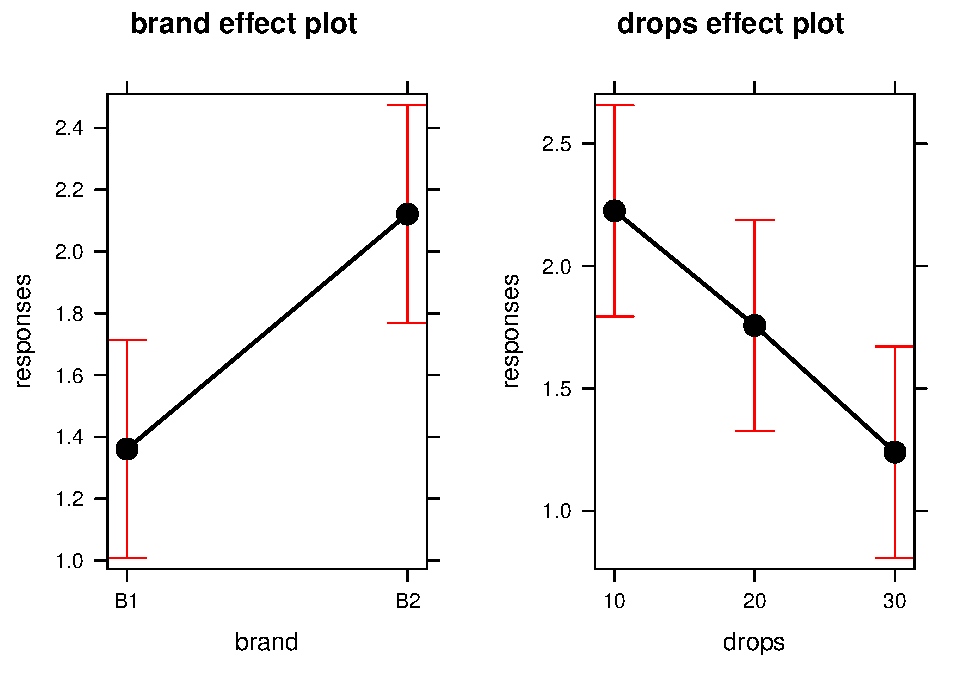
\includegraphics{04-twoWayAnova_files/figure-latex/Figure4-7-1.pdf}
\caption{\label{fig:Figure4-7}Term-plots of additive model for paper towel data. Left
panel displays results for two brands and right panel for number of
drops of water, each after controlling for the other.}
\end{figure}

\newpage

\section{Guinea pig tooth growth analysis with Two-Way
ANOVA}\label{section4-4}

The effects of dosage and delivery method of ascorbic acid on Guinea Pig
odontoblast growth was analyzed as a One-Way ANOVA in Section
\ref{section3-4} by assessing evidence of any difference in the means of
any combinations of dosage method (Vit C capsule vs Orange Juice) and
three dosage amounts (0.5, 1, and 2 mg/day). Now we will consider the
dosage and delivery methods as two separate variables and explore their
potential interaction. A beanplot and interaction plot are provided in
Figure \ref{fig:Figure4-8}.



\begin{figure}
\centering
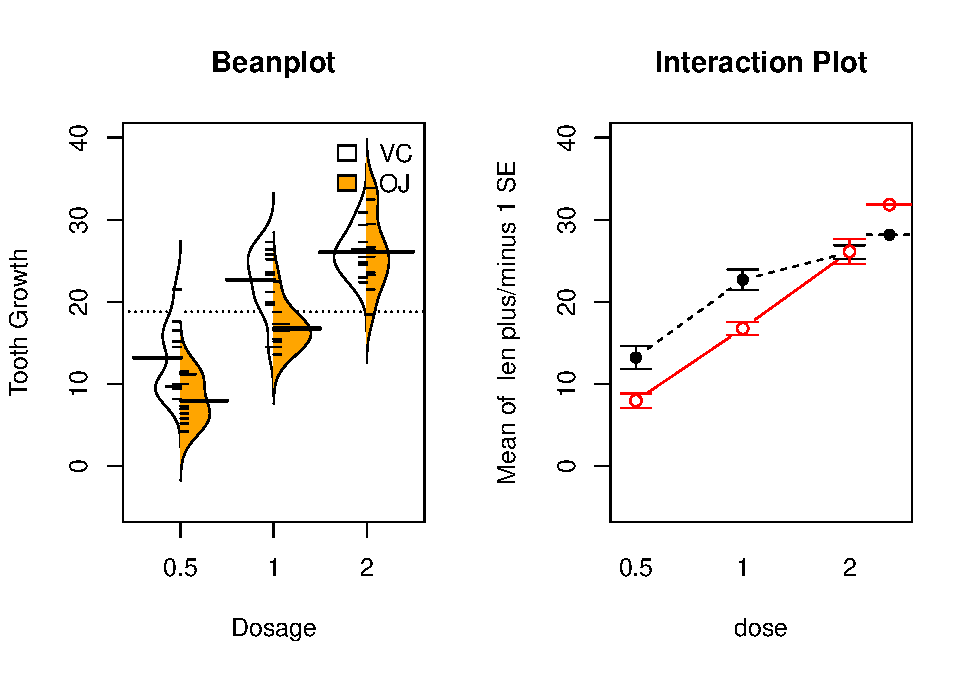
\includegraphics{04-twoWayAnova_files/figure-latex/Figure4-8-1.pdf}
\caption{\label{fig:Figure4-8}Beanplot and interaction plot of the tooth growth data set.}
\end{figure}

\begin{Shaded}
\begin{Highlighting}[]
\KeywordTok{data}\NormalTok{(ToothGrowth)}
\KeywordTok{par}\NormalTok{(}\DataTypeTok{mfrow=}\KeywordTok{c}\NormalTok{(}\DecValTok{1}\NormalTok{,}\DecValTok{2}\NormalTok{))}
\KeywordTok{beanplot}\NormalTok{(len }\OperatorTok{~}\StringTok{ }\NormalTok{supp}\OperatorTok{*}\NormalTok{dose, }\DataTypeTok{data=}\NormalTok{ToothGrowth, }\DataTypeTok{side=}\StringTok{"b"}\NormalTok{, }\DataTypeTok{ylim=}\KeywordTok{c}\NormalTok{(}\OperatorTok{-}\DecValTok{5}\NormalTok{,}\DecValTok{40}\NormalTok{),}
         \DataTypeTok{main=}\StringTok{"Beanplot"}\NormalTok{, }\DataTypeTok{col=}\KeywordTok{list}\NormalTok{(}\StringTok{"white"}\NormalTok{,}\StringTok{"orange"}\NormalTok{), }\DataTypeTok{xlab=}\StringTok{"Dosage"}\NormalTok{,}
         \DataTypeTok{ylab=}\StringTok{"Tooth Growth"}\NormalTok{)}
\KeywordTok{legend}\NormalTok{(}\StringTok{"bottomright"}\NormalTok{, }\DataTypeTok{bty=}\StringTok{"n"}\NormalTok{, }\KeywordTok{c}\NormalTok{(}\StringTok{"VC"}\NormalTok{,}\StringTok{"OJ"}\NormalTok{), }\DataTypeTok{fill=}\KeywordTok{c}\NormalTok{(}\StringTok{"white"}\NormalTok{,}\StringTok{"orange"}\NormalTok{))}
\KeywordTok{intplot}\NormalTok{(len }\OperatorTok{~}\StringTok{ }\NormalTok{supp}\OperatorTok{*}\NormalTok{dose, }\DataTypeTok{data=}\NormalTok{ToothGrowth, }\DataTypeTok{col=}\KeywordTok{c}\NormalTok{(}\DecValTok{1}\NormalTok{,}\DecValTok{2}\NormalTok{), }
        \DataTypeTok{main=}\StringTok{"Interaction Plot"}\NormalTok{, }\DataTypeTok{ylim=}\KeywordTok{c}\NormalTok{(}\OperatorTok{-}\DecValTok{5}\NormalTok{,}\DecValTok{40}\NormalTok{))}
\end{Highlighting}
\end{Shaded}

It appears that the effect of method changes based on the dosage as the
interaction plot seems to show some evidence of non-parallel lines.
Actually, it appears that the effect of delivery method is parallel for
doses 0.5 and 1.0 mg/day but that the effect of delivery method changes
for 2 mg/day.

We can use the ANOVA \(F\)-test for an interaction to assess whether the
interaction is ``real'' relative to the variability in the responses.
That is, is it larger than we would expect due to natural variation in
the data? If yes, then it is a real effect and we should account for it.
The following results fit the interaction model and provide an ANOVA
table.

\begin{Shaded}
\begin{Highlighting}[]
\NormalTok{TG1 <-}\StringTok{ }\KeywordTok{lm}\NormalTok{(len}\OperatorTok{~}\NormalTok{supp}\OperatorTok{*}\NormalTok{dose,}\DataTypeTok{data=}\NormalTok{ToothGrowth)}
\KeywordTok{Anova}\NormalTok{(TG1)}
\end{Highlighting}
\end{Shaded}

\begin{verbatim}
## Anova Table (Type II tests)
## 
## Response: len
##            Sum Sq Df  F value    Pr(>F)
## supp       205.35  1  12.3170 0.0008936
## dose      2224.30  1 133.4151 < 2.2e-16
## supp:dose   88.92  1   5.3335 0.0246314
## Residuals  933.63 56
\end{verbatim}

The R output is reporting an interaction test result of \(F(1,56)=5.3\)
with a p-value of 0.025. But this should raise a red flag since the
numerator degrees of freedom are not what we should expect of
\((K-1)*(J-1) = (2-1)*(3-1)=2\). This brings up an issue in R when
working with categorical variables. If the levels of a categorical
variable are entered numerically, R will treat them as quantitative
variables and not split out the different levels of the categorical
variable. To make sure that R treats categorical variables the correct
way, we should use the \texttt{factor} function on any variables that
are categorical but are coded numerically in the data set. The following
code creates a new variable called \texttt{dosef} using the function
that will help us obtain correct results from the linear model. The
re-run of the ANOVA table provides the correct analysis and the expected
\(df\) for the two rows of output involving \texttt{dosef}:

\begin{Shaded}
\begin{Highlighting}[]
\NormalTok{ToothGrowth}\OperatorTok{$}\NormalTok{dosef<-}\KeywordTok{factor}\NormalTok{(ToothGrowth}\OperatorTok{$}\NormalTok{dose)}
\NormalTok{TG2 <-}\StringTok{ }\KeywordTok{lm}\NormalTok{(len }\OperatorTok{~}\StringTok{ }\NormalTok{supp}\OperatorTok{*}\NormalTok{dosef, }\DataTypeTok{data=}\NormalTok{ToothGrowth)}
\KeywordTok{Anova}\NormalTok{(TG2)}
\end{Highlighting}
\end{Shaded}

\begin{verbatim}
## Anova Table (Type II tests)
## 
## Response: len
##             Sum Sq Df F value    Pr(>F)
## supp        205.35  1  15.572 0.0002312
## dosef      2426.43  2  92.000 < 2.2e-16
## supp:dosef  108.32  2   4.107 0.0218603
## Residuals   712.11 54
\end{verbatim}

The ANOVA \(F\)-test for an interaction between supplement type and
dosage level is \(F(2,54)= 4.107\) with a p-value of 0.022. So there
appears to be enough evidence to reject the null hypothesis of no
interaction between \emph{Dosage} and \emph{Delivery method}, supporting
a changing effect on tooth growth of dosage based on the delivery method
in the Guinea Pigs that were assigned.

Any similarities between this correct result and the previous WRONG
result are coincidence. I (Greenwood) once attended a Master's defense
where the results from a similar model were not as expected (small
p-values in places they didn't expect and large p-values in places where
they thought differences existed). During the presentation, the student
showed some ANOVA tables and the four level categorical variable had 1
numerator \(df\) in the ANOVA table. The student passed with major
revisions but had to re-run \textbf{all} the results and re-write
\textbf{all} of the conclusions\ldots{} So be careful to check the ANOVA
results (\(df\) and for the right number of expected model coefficients)
to make sure they match your expectations. This is one reason why you
will be learning to fill in ANOVA tables based on information about the
study so that you can be prepared to detect when your code has let you
down\footnote{Just so you don't think that perfect R code should occur
  on the first try, we have all made similarly serious coding mistakes
  even after accumulating more than decade of experience with R. It is
  finding those mistakes that matters.}. It is also a great reason to
explore term-plots and coefficient interpretations as that can also help
diagnose errors in model construction.

Getting back to the previous results, we now have enough background
information to more formally write up a focused interpretation of these
results. The 6+ hypothesis testing steps in this situation would be
focused on first identifying that the best analysis here is as a Two-Way
ANOVA situation (these data were analyzed in Chapter \ref{chapter3} as a
One-Way ANOVA but this version is better because it can explore whether
there is an interaction between delivery method and dosage). We will use
a 5\% significance level and start with assessing the evidence for an
interaction. If the interaction had not been dropped, we would have
reported the test for the interaction, re-fit the additive model and
used it to explore the main effect tests and estimates for \emph{Dose}
and \emph{Delivery method}.

\begin{enumerate}
\def\labelenumi{\arabic{enumi}.}
\item
  \textbf{Hypotheses:}

  \begin{itemize}
  \tightlist
  \item
    \(H_0\): No interaction between \emph{Delivery method} and
    \emph{Dose} on odontoblast growth in population of guinea pigs
  \end{itemize}

  \(\Leftrightarrow\) All \(\omega_{jk}\text{'s}=0\).

  \begin{itemize}
  \tightlist
  \item
    \(H_A\): Interaction between \emph{Delivery method} and \emph{Dose}
    on odontoblast growth in population of guinea pigs
  \end{itemize}

  \(\Leftrightarrow\) At least one \(\omega_{jk}\ne 0\).
\item
  \textbf{Validity conditions:}

  \begin{itemize}
  \item
    Independence:

    \begin{itemize}
    \tightlist
    \item
      This assumption is presumed to be met because we don't know of a
      reason why the independence of the measurements of tooth growth of
      the guinea pigs as studied might be violated.
    \end{itemize}
  \item
    Constant variance:

    \begin{itemize}
    \item
      To assess this assumption, we can use the diagnostic plots in
      Figure \ref{fig:Figure4-9}.
    \item
      In the Residuals vs Fitted and the Scale-Location plots, the
      differences in variability among the groups (see the different
      x-axis positions for each group's fitted values) is minor, so
      there is not strong evidence of a problem with the equal variance
      assumption.
    \end{itemize}

    \begin{figure}
    \centering
    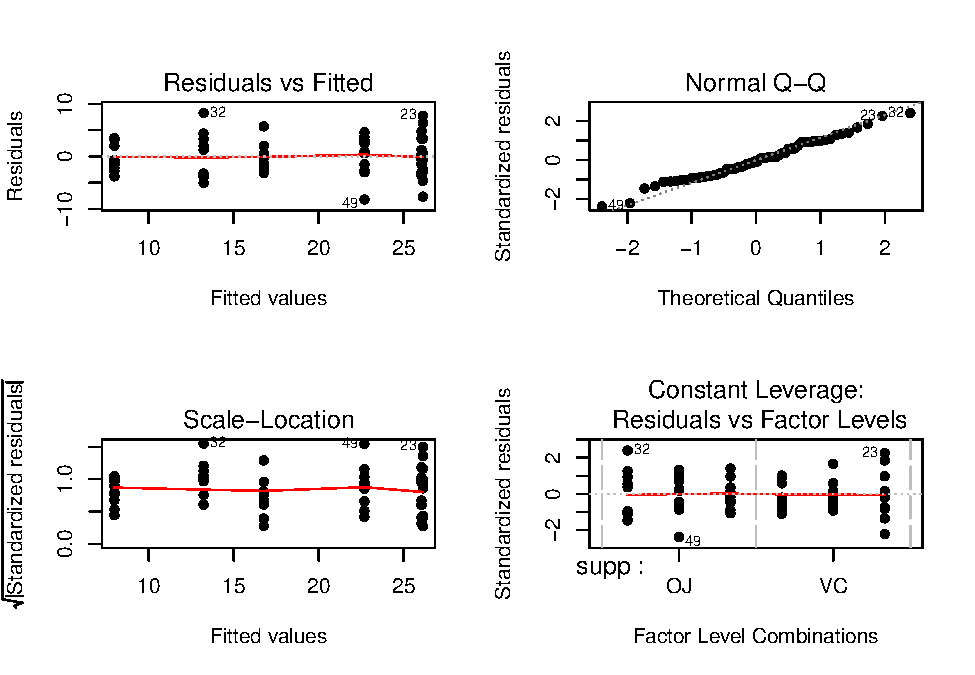
\includegraphics{04-twoWayAnova_files/figure-latex/Figure4-9-1.pdf}
    \caption{\label{fig:Figure4-9}Diagnostic plots for the interaction model
    for Tooth Growth.}
    \end{figure}

\begin{Shaded}
\begin{Highlighting}[]
\KeywordTok{par}\NormalTok{(}\DataTypeTok{mfrow=}\KeywordTok{c}\NormalTok{(}\DecValTok{2}\NormalTok{,}\DecValTok{2}\NormalTok{))}
\KeywordTok{plot}\NormalTok{(TG2, }\DataTypeTok{pch=}\DecValTok{16}\NormalTok{) }
\end{Highlighting}
\end{Shaded}
  \item
    Normality of residuals:

    \begin{itemize}
    \tightlist
    \item
      The QQ-Plot in Figure \ref{fig:Figure4-9} does not suggest a
      problem with this assumption.
    \end{itemize}
  \end{itemize}
\end{enumerate}

\newpage

\begin{enumerate}
\def\labelenumi{\arabic{enumi}.}
\setcounter{enumi}{2}
\item
  \textbf{Calculate the test statistic for the Interaction test.}

\begin{Shaded}
\begin{Highlighting}[]
\NormalTok{TG2 <-}\StringTok{ }\KeywordTok{lm}\NormalTok{(len }\OperatorTok{~}\StringTok{ }\NormalTok{supp}\OperatorTok{*}\NormalTok{dosef, }\DataTypeTok{data=}\NormalTok{ToothGrowth)}
\KeywordTok{Anova}\NormalTok{(TG2) }
\end{Highlighting}
\end{Shaded}

\begin{verbatim}
## Anova Table (Type II tests)
## 
## Response: len
##             Sum Sq Df F value    Pr(>F)
## supp        205.35  1  15.572 0.0002312
## dosef      2426.43  2  92.000 < 2.2e-16
## supp:dosef  108.32  2   4.107 0.0218603
## Residuals   712.11 54
\end{verbatim}

  \begin{itemize}
  \tightlist
  \item
    The test statistic is \(F(2,54)=4.107\).
  \end{itemize}
\item
  \textbf{Find the p-value:}

  \begin{itemize}
  \item
    The ANOVA \(F\)-test p-value of 0.0219 for the interaction.
  \item
    To find this p-value directly in R, we can use the \texttt{pf}
    function.
  \end{itemize}

\begin{Shaded}
\begin{Highlighting}[]
\KeywordTok{pf}\NormalTok{(}\FloatTok{4.107}\NormalTok{, }\DataTypeTok{df1=}\DecValTok{2}\NormalTok{, }\DataTypeTok{df2=}\DecValTok{54}\NormalTok{, }\DataTypeTok{lower.tail=}\NormalTok{F)}
\end{Highlighting}
\end{Shaded}

\begin{verbatim}
## [1] 0.0218601
\end{verbatim}
\item
  \textbf{Make a decision:}

  \begin{itemize}
  \tightlist
  \item
    Reject \(H_0\) since the p-value (0.0219) is less than 0.05. With a
    p-value of 0.0219, there is about a 2.19\% chance we would observe
    interaction like we did (or more extreme) if none were truly
    present. This provides strong evidence against the null hypothesis
    of no interaction between delivery method and dosage on odontoblast
    growth so we reject the null hypothesis of no interaction.
  \end{itemize}
\item
  \textbf{Write a conclusion:}

  \begin{itemize}
  \tightlist
  \item
    Therefore, the effects of dosage level (0.5, 1, or 2 mg/day) on
    population average tooth odontoblast growth rates of Guinea pigs are
    changed by the delivery (OJ, Vitamin C) method (and vice versa) and
    we should keep the interaction in the model. With the random
    assignment of levels but not random selection of subjects here, we
    could also write this as: Different dosage levels cause different
    changes in the odontoblast growth based on the delivery method for
    these guinea pigs.
  \end{itemize}
\end{enumerate}

In a Two-Way ANOVA, we need to go a little further to get to the final
interpretations since the models are more complicated. When there is an
interaction present, we should focus on the interaction plot or
term-plot of the interaction model for an interpretation of the form and
pattern of the interaction. If the interaction were unimportant, then
the hypotheses and results should focus on the additive model results,
especially the estimated model coefficients. To see why we don't spend
much time with the estimated model coefficients in an interaction model,
the model summary for this model is provided:

\begin{Shaded}
\begin{Highlighting}[]
\KeywordTok{summary}\NormalTok{(TG2)}
\end{Highlighting}
\end{Shaded}

\begin{verbatim}
## 
## Call:
## lm(formula = len ~ supp * dosef, data = ToothGrowth)
## 
## Residuals:
##    Min     1Q Median     3Q    Max 
##  -8.20  -2.72  -0.27   2.65   8.27 
## 
## Coefficients:
##               Estimate Std. Error t value Pr(>|t|)
## (Intercept)     13.230      1.148  11.521 3.60e-16
## suppVC          -5.250      1.624  -3.233  0.00209
## dosef1           9.470      1.624   5.831 3.18e-07
## dosef2          12.830      1.624   7.900 1.43e-10
## suppVC:dosef1   -0.680      2.297  -0.296  0.76831
## suppVC:dosef2    5.330      2.297   2.321  0.02411
## 
## Residual standard error: 3.631 on 54 degrees of freedom
## Multiple R-squared:  0.7937, Adjusted R-squared:  0.7746 
## F-statistic: 41.56 on 5 and 54 DF,  p-value: < 2.2e-16
\end{verbatim}

There are two \(\omega_{jk}\text{'s}\) in the results, related to
modifying the estimates for doses of 1 (-0.68) and 2 (5.33) for the
Vitamin C group. If you want to re-construct the fitted values from the
model that are displayed in the Figure \ref{fig:Figure4-10}, you have to
look for any coefficients that are ``turned on'' for a combination of
levels of interest. For example, for the OJ group (solid line in Figure
\ref{fig:Figure4-10}), the dosage of 0.5 mg/day has an estimate of an
average growth of approximately 13 mm. This is the baseline group, so
the model estimate for an observation in the OJ and 0.5 mg/day dosage is
simply \(\hat{y}_{i,\text{OJ},0.5mg}=\hat{\alpha}=13.23\) microns. For
the OJ and 2 mg dosage estimate that has a value over 25 microns in the
plot, the model incorporates the deviation for the 2 mg dosage:
\(\hat{y}_{i,\text{OJ},2mg}=\hat{\alpha} + \hat{\tau}_{2mg}=13.23 + 12.83 = 26.06\)
microns. For the Vitamin C group, another coefficient becomes involved
from its ``main effect''. For the VC and 0.5 mg dosage level, the
estimate is approximately 8 microns. The pertinent model components are
\(\hat{y}_{i,\text{VC},0.5mg}=\hat{\alpha} + \hat{\gamma}_{\text{VC}}=13.23 + (-5.25) = 7.98\)
microns. Finally, when we consider non-baseline results for both groups,
three coefficients are required to reconstruct the results in the plot.
For example, the estimate for the VC, 1 mg dosage is
\(\hat{y}_{i,\text{VC},1mg}=\hat{\alpha} + \hat{\tau}_{1mg} + \hat{\gamma}_{\text{VC}} =13.23 + 9.47 + (-5.25) = 17.45\)
microns. We usually will by-pass all this fun(!) with the coefficients
in an interaction model and go from the ANOVA interaction test to
focusing on the pattern of the responses in the interaction plot, but it
is good to know that there are still model coefficients driving our
results.




\begin{figure}
\centering
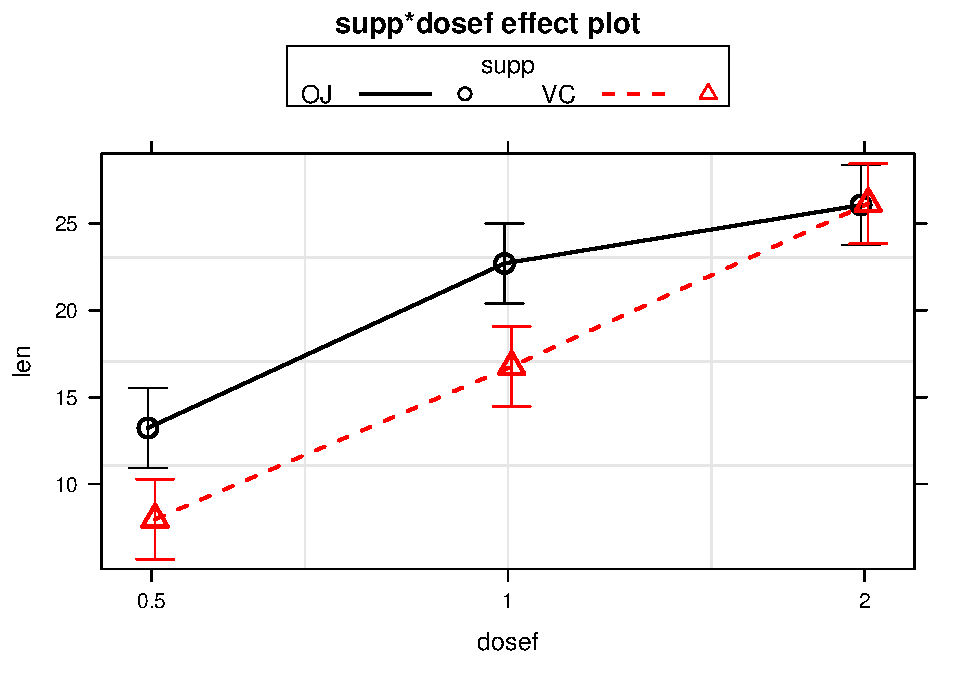
\includegraphics{04-twoWayAnova_files/figure-latex/Figure4-10-1.pdf}
\caption{\label{fig:Figure4-10}Term-plot for the estimated interaction for the Tooth
Growth data.}
\end{figure}



\begin{figure}
\centering
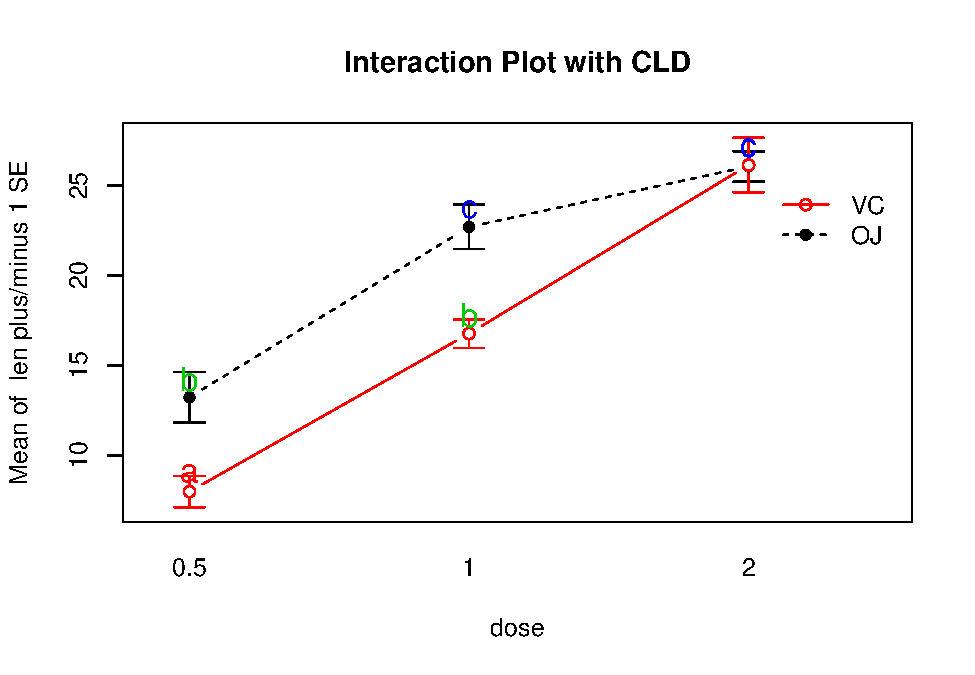
\includegraphics{04-twoWayAnova_files/figure-latex/Figure4-11-1.pdf}
\caption{\label{fig:Figure4-11}Interaction plot with added CLD from Tukey's HSD.}
\end{figure}

\begin{Shaded}
\begin{Highlighting}[]
\KeywordTok{plot}\NormalTok{(}\KeywordTok{allEffects}\NormalTok{(TG2), }\DataTypeTok{grid=}\NormalTok{T, }\DataTypeTok{multiline=}\NormalTok{T, }\DataTypeTok{ci.style=}\StringTok{"bars"}\NormalTok{)}
\end{Highlighting}
\end{Shaded}

Given the presence of an important interaction, then the final step in
the interpretation here is to interpret the results in the interaction
plot or term-plot of the interaction model, supported by the p-value
suggesting evidence of a different effect of supplement type based on
the dosage level. To supplement this even more, knowing which
combinations of levels differ can enhance our discussion. Tukey's HSD
results (specifically the CLD) can be added to the original interaction
plot by turning on the \texttt{cld=T} option in the \texttt{intplot}
function as seen in Figure \ref{fig:Figure4-11}. Sometimes it is hard to
see the letters and so there is also a \texttt{cldshift=...} option to
move the letters up or down, here a value of 1 seemed to work.

\begin{Shaded}
\begin{Highlighting}[]
\KeywordTok{intplot}\NormalTok{(len }\OperatorTok{~}\StringTok{ }\NormalTok{supp}\OperatorTok{*}\NormalTok{dose, }\DataTypeTok{data=}\NormalTok{ToothGrowth, }\DataTypeTok{col=}\KeywordTok{c}\NormalTok{(}\DecValTok{1}\NormalTok{,}\DecValTok{2}\NormalTok{), }\DataTypeTok{cldshift=}\DecValTok{1}\NormalTok{,}
        \DataTypeTok{cld=}\NormalTok{T, }\DataTypeTok{main=}\StringTok{"Interaction Plot with CLD"}\NormalTok{)}
\end{Highlighting}
\end{Shaded}

The interpretation of the previous hypothesis test result can be
concluded with the following discussion. Generally increasing the dosage
increases the amount of mean growth except for the 2 mg/day dosage level
where the increase levels off in the OJ group (OJ 1 and 2 mg/day are not
detectably different) and the differences between the two delivery
methods disappear at the highest dosage level. But for 0.5 and 1 mg/day
dosages, OJ is clearly better than VC by about 10 microns of growth on
average.

\section{Observational study example: The Psychology of
Debt}\label{section4-5}

In this section, the analysis of a survey of \(N=464\) randomly sampled
adults will be analyzed from a survey conducted by \citet{Lea1995} and
available in the \texttt{debt} data set from the \texttt{faraway}
package \citep{R-faraway}. The subjects responded to a variety of
questions including whether they buy cigarettes (\texttt{cigbuy}: 0 if
no, 1 if yes), their housing situation (\texttt{house}: 1 = rent, 2 =
mortgage, and 3 = owned outright), their income group
(\texttt{incomegp}: 1 = lowest, 5 = highest), and their score on a
continuous scale of attitudes about debt (\texttt{prodebt}: 1 = least
favorable, 5 = most favorable). \texttt{prodebt} was derived as the
average of a series of questions about debt with each question measured
on an \textbf{\emph{ordinal}} 1 to 5 scale, with higher values
corresponding to more positive responses about \textbf{going into debt}
of various kinds. The ordered scale on surveys that try to elicit your
opinions on topics with scales from 1 to 5 or 1 to 7 or even, sometimes,
1 to 10 is called a \textbf{\emph{Likert scale}} \citep{Likert1932}. It
is not a quantitative scale and really should be handled more carefully
than taking an average of a set responses. That said, it is extremely
common practice in social science research to treat ordinal responses as
if they are quantitative and take the average of many of them to create
a more continuous response variable like the one we are using here. If
you continue your statistics explorations, you will see some better
techniques for analyzing responses obtained in this fashion. That said,
the scale of the response is relatively easy to understand as an amount
of willingness to go into debt on a scale from 1 to 5 with higher values
corresponding to more willingness to be in debt.

This data set is typical of survey data where respondents were not
required to answer all questions and there are some missing responses.
We will clean out any individuals that failed to respond to all
questions using the \texttt{na.omit} function, which will return only
subjects that responded to every question in the data set. But is this
dangerous? Suppose that people did not want to provide their income
levels if they were in the lowest or, maybe, highest income groups. Then
we would be missing responses systematically and conclusions could be
biased because of ignoring these types of subjects. This is another
topic for more advanced statistical methods to try to handle but
something every researcher should worry about when selected subjects do
not respond at all or fail to answer some questions. Is there bias
because of responses that were not observed that could invalidate all my
hard won statistical conclusions? This ties back into our discussion of
who was sampled. We need to think carefully about who was part of the
sample but refused to participate and how that might impact our
inferences.

Ignoring this potential for bias in the results for the moment, we are
first interested in whether buying cigarettes/not and income groups
interact in their explanation of the respondent's mean opinions on being
in debt. The interaction plot (Figure \ref{fig:Figure4-12}) may suggest
an interaction between \texttt{cigbuy} and \texttt{incomegp} from income
levels 1 to 3 where the lines cross but it is not as clear as the
previous examples. The interaction \(F\)-test helps us objectively
assess evidence for that interaction. Based on the plot, there do not
appear to be differences based on cigarette purchasing but there might
be some differences between the income groups. If there is no
interaction present, then this suggests that we might be in Scenario 2
or 3 where a single main effect of interest is present.

\begin{Shaded}
\begin{Highlighting}[]
\KeywordTok{require}\NormalTok{(faraway)}
\KeywordTok{data}\NormalTok{(debt)}
\NormalTok{debt}\OperatorTok{$}\NormalTok{incomegp <-}\StringTok{ }\KeywordTok{factor}\NormalTok{(debt}\OperatorTok{$}\NormalTok{incomegp)}
\NormalTok{debt}\OperatorTok{$}\NormalTok{cigbuy <-}\StringTok{ }\KeywordTok{factor}\NormalTok{(debt}\OperatorTok{$}\NormalTok{cigbuy)}
\NormalTok{debtc <-}\StringTok{ }\KeywordTok{na.omit}\NormalTok{(debt)}
\end{Highlighting}
\end{Shaded}




\begin{figure}
\centering
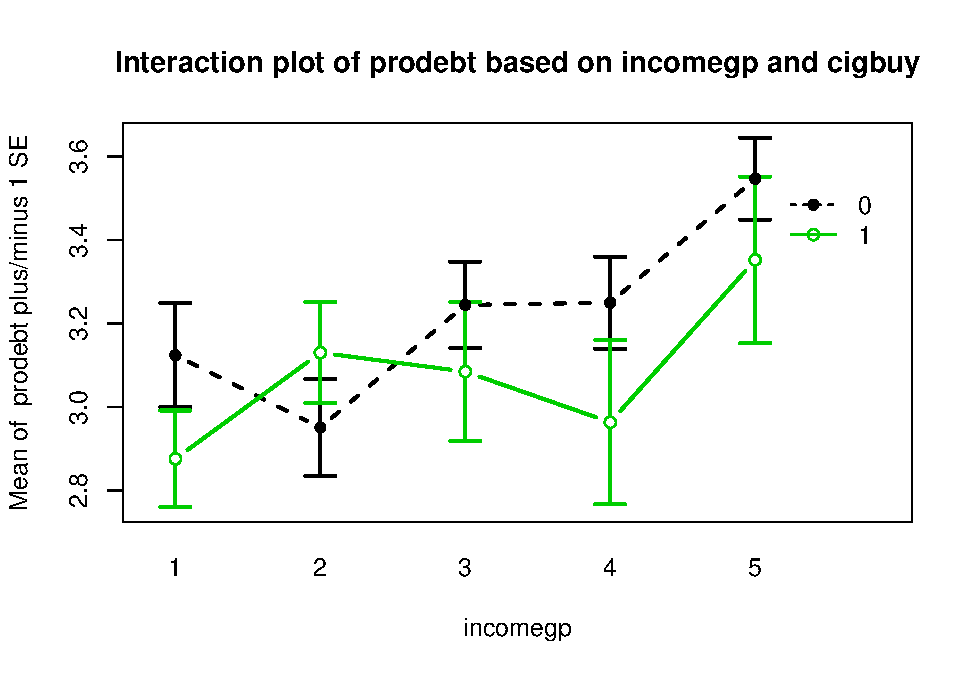
\includegraphics{04-twoWayAnova_files/figure-latex/Figure4-12-1.pdf}
\caption{\label{fig:Figure4-12}Interaction plot of \texttt{prodebt} by income group and
buy cigarettes (0=no, 1=yes).}
\end{figure}

\begin{Shaded}
\begin{Highlighting}[]
\KeywordTok{intplot}\NormalTok{(prodebt }\OperatorTok{~}\StringTok{ }\NormalTok{cigbuy}\OperatorTok{*}\NormalTok{incomegp, }\DataTypeTok{data=}\NormalTok{debtc, }\DataTypeTok{col=}\KeywordTok{c}\NormalTok{(}\DecValTok{1}\NormalTok{,}\DecValTok{3}\NormalTok{), }\DataTypeTok{lwd=}\DecValTok{2}\NormalTok{)}
\end{Highlighting}
\end{Shaded}

As in other situations, and especially with observational studies where
a single large sample is analyzed, it is important to check for balance
- whether all the combinations of the two predictor variables are
similarly represented. Even more critically, we need to check whether
all the combinations of levels of factors are measured. If a combination
is not measured, then we lose the ability to estimate the mean for that
combination and the ability to test for an interaction. A solution to
that problem would be to collapse the categories of one of the
variables, changing the definitions of the levels but if you fail to
obtain information for all combinations, you can't work with the
interaction model. In this situation, we barely have enough information
to proceed (the smallest \(n_{jk}\) is 8 for income group 4 that buys
cigarettes). We have a very unbalanced design with counts between 8 and
51 in the different combinations.

\begin{Shaded}
\begin{Highlighting}[]
\KeywordTok{tally}\NormalTok{(cigbuy }\OperatorTok{~}\StringTok{ }\NormalTok{incomegp, }\DataTypeTok{data=}\NormalTok{debtc)}
\end{Highlighting}
\end{Shaded}

\begin{verbatim}
##       incomegp
## cigbuy  1  2  3  4  5
##      0 24 40 45 47 51
##      1 23 29 18  8 19
\end{verbatim}

The test for the interaction is always how we start our modeling in
Two-Way ANOVA situations. The ANOVA table suggests that there is little
evidence of interaction between the income level and buying cigarettes
on the opinions of the respondents towards debt (\(F(4,294)=1.0003\),
p-value=0.408). This suggests that the initial assessment that the
interaction wasn't too prominent was correct. We should move to the
additive model here but first need to check the assumptions to make sure
we can trust this initial test.

\begin{Shaded}
\begin{Highlighting}[]
\KeywordTok{require}\NormalTok{(car)}
\NormalTok{debt1 <-}\StringTok{ }\KeywordTok{lm}\NormalTok{(prodebt }\OperatorTok{~}\StringTok{ }\NormalTok{incomegp}\OperatorTok{*}\NormalTok{cigbuy, }\DataTypeTok{data=}\NormalTok{debtc)}
\KeywordTok{Anova}\NormalTok{(debt1)}
\end{Highlighting}
\end{Shaded}

\begin{verbatim}
## Anova Table (Type II tests)
## 
## Response: prodebt
##                  Sum Sq  Df F value   Pr(>F)
## incomegp          9.018   4  4.5766 0.001339
## cigbuy            0.703   1  1.4270 0.233222
## incomegp:cigbuy   1.971   4  1.0003 0.407656
## Residuals       144.835 294
\end{verbatim}

The diagnostic plots (Figure \ref{fig:Figure4-13}) seem to be pretty
well-behaved with no apparent violations of the normality assumption and
no clear evidence of a violation of the constant variance assumption.
The observations would seem to be independent because there is no
indication of structure to the measurements of the survey respondents
that might create dependencies. In observational studies, violations of
the independence assumption might come from repeated measures of the
same person or multiple measurements within the same family/household or
samples that are clustered geographically. The random sampling from a
population should allow inferences to a larger population except for
that issue of removing partially missing responses. We also don't have
much information on the population sampled, so will just leave this
vague here but know that there is a population these conclusions apply
to since it was random sample. All of this suggests proceeding to
fitting and exploring the additive model is reasonable here. No causal
inferences are possible because this is an observational study.




\begin{figure}
\centering
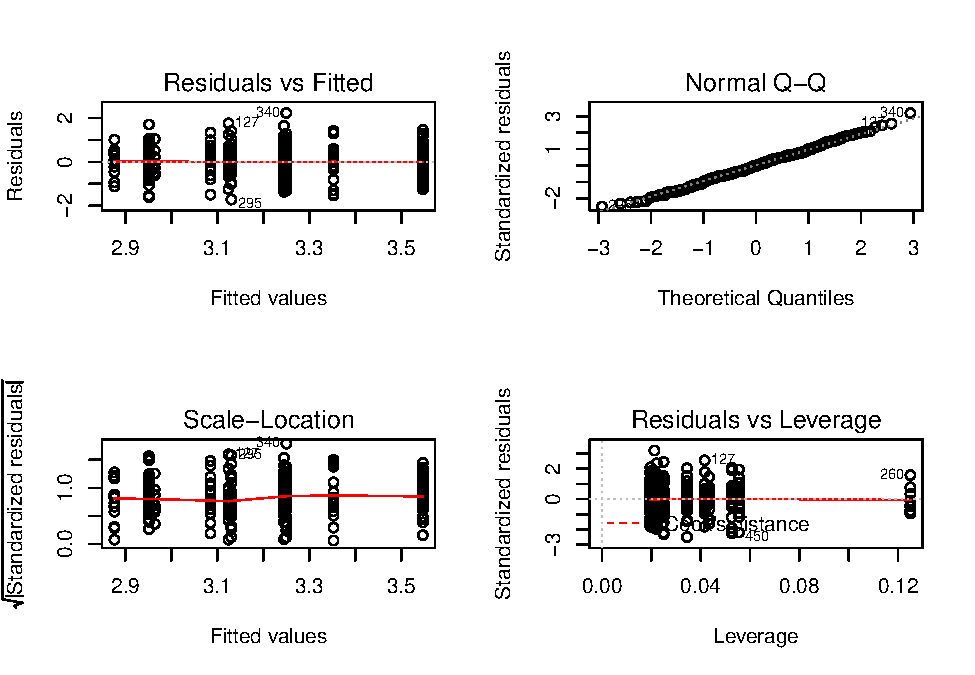
\includegraphics{04-twoWayAnova_files/figure-latex/Figure4-13-1.pdf}
\caption{\label{fig:Figure4-13}Diagnostic plot for \texttt{prodebt} by income group and
buy cigarettes/not interaction model.}
\end{figure}

\begin{Shaded}
\begin{Highlighting}[]
\KeywordTok{par}\NormalTok{(}\DataTypeTok{mfrow=}\KeywordTok{c}\NormalTok{(}\DecValTok{2}\NormalTok{,}\DecValTok{2}\NormalTok{))}
\KeywordTok{plot}\NormalTok{(debt1)}
\end{Highlighting}
\end{Shaded}

\begin{enumerate}
\def\labelenumi{\arabic{enumi}.}
\item
  \textbf{Hypotheses (Two sets apply when the additive model is the
  focus!):}

  \begin{itemize}
  \tightlist
  \item
    \(H_0\): No difference in means for \texttt{prodebt} for income
    groups in population, given cigarette buying in model
  \end{itemize}

  \(\Leftrightarrow\) All \(\tau_j\text{'s} = 0\) in additive model.

  \begin{itemize}
  \tightlist
  \item
    \(H_A\): Some difference in means for \texttt{prodebt} for income
    group in population, given cigarette buying in model
  \end{itemize}

  \(\Leftrightarrow\) Not all \(\tau_j\text{'s} = 0\) in additive model.

  \begin{itemize}
  \tightlist
  \item
    \(H_0\): No difference in means for \texttt{prodebt} for cigarette
    buying/not in population, given income group in model 
  \end{itemize}

  \(\Leftrightarrow\) All \(\gamma_k\text{'s} = 0\) in additive model.

  \begin{itemize}
  \tightlist
  \item
    \(H_A\): Some difference in means for \texttt{prodebt} for cigarette
    buying/not in population, given income group in model
  \end{itemize}

  \(\Leftrightarrow\) Not all \(\gamma_k\text{'s} = 0\) in additive
  model.
\item
  \textbf{Validity conditions -- discussed above but with new plots for
  the additive:}

  \begin{figure}
  \centering
  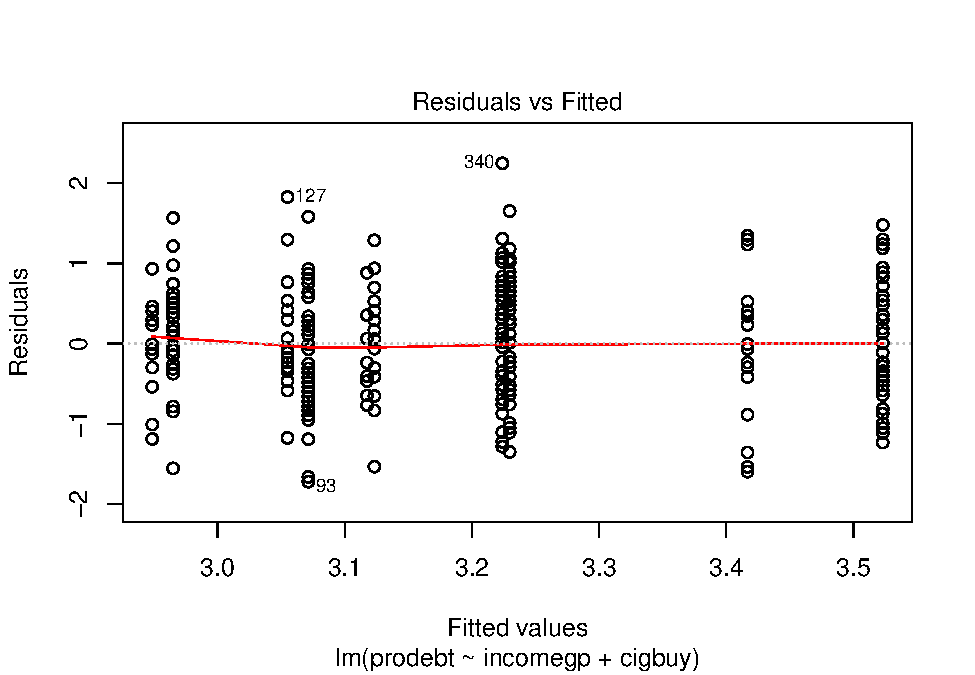
\includegraphics{04-twoWayAnova_files/figure-latex/Figure4-14-1.pdf}
  \caption{\label{fig:Figure4-14}Diagnostic plot for \texttt{prodebt} by
  income group and buy cigarettes/not}
  \end{figure}

\begin{Shaded}
\begin{Highlighting}[]
\NormalTok{debt1r<-}\KeywordTok{lm}\NormalTok{(prodebt}\OperatorTok{~}\NormalTok{incomegp}\OperatorTok{+}\NormalTok{cigbuy,}\DataTypeTok{data=}\NormalTok{debtc)}
\KeywordTok{plot}\NormalTok{(debt1r)}
\end{Highlighting}
\end{Shaded}

  \begin{itemize}
  \item
    Constant Variance:

    \begin{itemize}
    \tightlist
    \item
      In the Residuals vs Fitted and the Scale-Location plots in Figure
      \ref{fig:Figure4-14}, the differences in variability among groups
      is minor and nothing suggests a violation. \textbf{If you change
      models, you should always revisit the diagnostic plots to make
      sure you didn't create problems that were not present in more
      complicated models.}
    \end{itemize}
  \item
    Normality of residuals:

    \begin{itemize}
    \tightlist
    \item
      The QQ-Plot in Figure \ref{fig:Figure4-14} does not suggest a
      problem with this assumption.
    \end{itemize}
  \end{itemize}
\item
  \textbf{Calculate the test statistic for the two main effect tests.}

\begin{Shaded}
\begin{Highlighting}[]
\KeywordTok{Anova}\NormalTok{(debt1r)}
\end{Highlighting}
\end{Shaded}

\begin{verbatim}
## Anova Table (Type II tests)
## 
## Response: prodebt
##            Sum Sq  Df F value   Pr(>F)
## incomegp    9.018   4  4.5766 0.001335
## cigbuy      0.703   1  1.4270 0.233210
## Residuals 146.806 298
\end{verbatim}

  \begin{itemize}
  \tightlist
  \item
    The test statistics are \(F(4,298)=4.577\) and \(F(1,298)=1.427\).
  \end{itemize}
\item
  \textbf{Find the p-value:}

  \begin{itemize}
  \tightlist
  \item
    The ANOVA \(F\)-test p-values are 0.001335 for the income group
    variable (conditional on cigarette buy) and 0.2232 for the cigarette
    buy variable (conditional on income group).
  \end{itemize}
\item
  \textbf{Make decisions:}

  \begin{itemize}
  \tightlist
  \item
    Reject \(H_0\) of no income group differences (p-value=0.0013) and
    fail to reject \(H_0\) of no cigarette buying differences
    (p-value=0.2232), each after controlling for the other variable.
  \end{itemize}
\item
  \textbf{Write a conclusion:}

  \begin{itemize}
  \tightlist
  \item
    There was initially no evidence to support retaining the interaction
    of income group and cigarette buying on pro-debt feelings
    (\(F(4,294)=1.00, \text{p-value} =0.408\)) so the interaction was
    dropped from the model. There is strong evidence of some difference
    in the mean pro-debt feelings in the population across the income
    groups, after adjusting for cigarette buying. There is little to no
    evidence of a difference in the mean pro-debt feelings in the
    population based on cigarette buying/not, after adjusting for income
    group.
  \end{itemize}
\end{enumerate}

So we learned that the additive model was more appropriate for these
responses and that the results resemble Scenario 2 or 3 with only one
main effect being important. In the additive model, the coefficients can
be interpreted as shifts from the baseline after controlling for the
other variable in the model. Figure \ref{fig:Figure4-15} shows the
increasing average comfort with being in debt as the income groups go
up. Being a cigarette buyer was related to a lower comfort level with
debt. But compare the y-axis scales in the two plots -- the differences
in the means across income groups are almost 0.5 points on a 5 point
scale whereas the difference across \texttt{cigbuy}'s two levels is less
than 0.15 units. The error bars for the 95\% confidence intervals are of
similar width but the differences in means show up clearly in the income
group term-plot. This is all indirectly related to the size of the
p-values for each term in the additive model but hopefully helps to
build some intuition on the reason for differences.





\begin{Shaded}
\begin{Highlighting}[]
\KeywordTok{plot}\NormalTok{(}\KeywordTok{allEffects}\NormalTok{(debt1r))}
\end{Highlighting}
\end{Shaded}

\begin{figure}
\centering
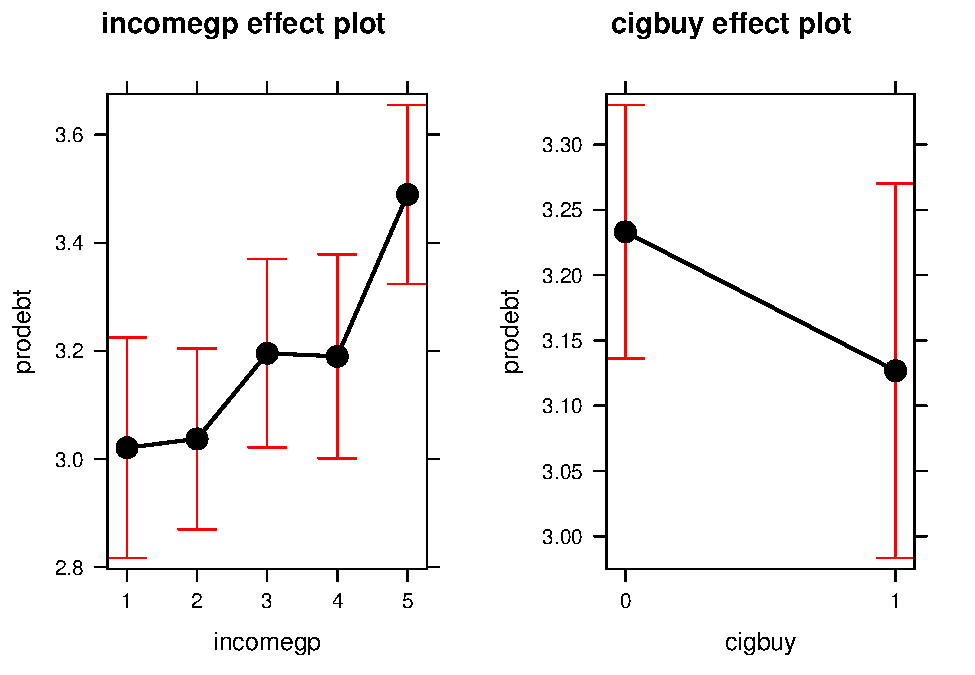
\includegraphics{04-twoWayAnova_files/figure-latex/Figure4-15-1.pdf}
\caption{\label{fig:Figure4-15}Term-plots for the \texttt{prodebt} additive model with
left panel for income group and the right panel for buying cigarettes or
not (1 for yes).}
\end{figure}

The estimated coefficients can also be interesting to interpret for the
additive model. Here are the model summary coefficients:

\begin{Shaded}
\begin{Highlighting}[]
\KeywordTok{summary}\NormalTok{(debt1r)}\OperatorTok{$}\NormalTok{coefficients}
\end{Highlighting}
\end{Shaded}

\begin{verbatim}
##                Estimate Std. Error    t value     Pr(>|t|)
## (Intercept)  3.05483517 0.11127284 27.4535561 1.357428e-83
## incomegp2    0.01640636 0.13288796  0.1234601 9.018260e-01
## incomegp3    0.17477182 0.13649309  1.2804444 2.013846e-01
## incomegp4    0.16900515 0.14274836  1.1839376 2.373813e-01
## incomegp5    0.46833117 0.13377661  3.5008449 5.347171e-04
## cigbuy1     -0.10640228 0.08907259 -1.1945569 2.332101e-01
\end{verbatim}

In the model, the baseline group is for non-cigarette buyers
(\texttt{cigbuy=0}) and income group 1 with \(\hat{\alpha}= 3.055\)
points. Regardless of the \texttt{cigbuy} level, the difference between
income groups 2 and 1 is estimated to be \(\hat{\tau}_2=0.016\), an
increase in the mean score of 0.016 points. Similarly, the difference
between income groups 3 and 1 is \(\hat{\tau}_3=0.175\) points,
regardless of cigarette smoking status. The estimated difference between
cigarette buyers and non-buyers was estimated as
\(\hat{\gamma}_2=-0.106\) points for any income group, remember that
this variable had a moderately large p-value in this model. The additive
model-based estimates for all six combinations can be found in Table
\ref{tab:Table4-3}.




\small

\begin{longtable}[]{@{}llllll@{}}
\caption{\label{tab:Table4-3} Calculations to construct the estimates for all
combinations of variables for the \texttt{prodebt} additive model.}\tabularnewline
\toprule
\begin{minipage}[b]{0.12\columnwidth}\raggedright\strut
\(\color{red}{\text{Cig}}\)\\
\(\color{red}{\text{Buy}}\)\strut
\end{minipage} & \begin{minipage}[b]{0.12\columnwidth}\raggedright\strut
\(\color{blue}{\textbf{Income}}\)\\
\(\color{blue}{\textbf{Group 1}}\)\strut
\end{minipage} & \begin{minipage}[b]{0.15\columnwidth}\raggedright\strut
\(\color{blue}{\textbf{Income}}\)\\
\(\color{blue}{\textbf{Group 2}}\)\strut
\end{minipage} & \begin{minipage}[b]{0.15\columnwidth}\raggedright\strut
\(\color{blue}{\textbf{Income}}\)\\
\(\color{blue}{\textbf{Group 3}}\)\strut
\end{minipage} & \begin{minipage}[b]{0.15\columnwidth}\raggedright\strut
\(\color{blue}{\textbf{Income}}\)\\
\(\color{blue}{\textbf{Group 4}}\)\strut
\end{minipage} & \begin{minipage}[b]{0.15\columnwidth}\raggedright\strut
\(\color{blue}{\textbf{Income}}\)\\
\(\color{blue}{\textbf{Group 5}}\)\strut
\end{minipage}\tabularnewline
\midrule
\endfirsthead
\toprule
\begin{minipage}[b]{0.12\columnwidth}\raggedright\strut
\(\color{red}{\text{Cig}}\)\\
\(\color{red}{\text{Buy}}\)\strut
\end{minipage} & \begin{minipage}[b]{0.12\columnwidth}\raggedright\strut
\(\color{blue}{\textbf{Income}}\)\\
\(\color{blue}{\textbf{Group 1}}\)\strut
\end{minipage} & \begin{minipage}[b]{0.15\columnwidth}\raggedright\strut
\(\color{blue}{\textbf{Income}}\)\\
\(\color{blue}{\textbf{Group 2}}\)\strut
\end{minipage} & \begin{minipage}[b]{0.15\columnwidth}\raggedright\strut
\(\color{blue}{\textbf{Income}}\)\\
\(\color{blue}{\textbf{Group 3}}\)\strut
\end{minipage} & \begin{minipage}[b]{0.15\columnwidth}\raggedright\strut
\(\color{blue}{\textbf{Income}}\)\\
\(\color{blue}{\textbf{Group 4}}\)\strut
\end{minipage} & \begin{minipage}[b]{0.15\columnwidth}\raggedright\strut
\(\color{blue}{\textbf{Income}}\)\\
\(\color{blue}{\textbf{Group 5}}\)\strut
\end{minipage}\tabularnewline
\midrule
\endhead
\begin{minipage}[t]{0.12\columnwidth}\raggedright\strut
\(\color{red}{\text{0:No}}\)\strut
\end{minipage} & \begin{minipage}[t]{0.12\columnwidth}\raggedright\strut
\(\hat{\alpha} ={\small 3.055}\)\strut
\end{minipage} & \begin{minipage}[t]{0.15\columnwidth}\raggedright\strut
\(\hat{\alpha} + \hat{\tau}_2\)\\
\(=3.055 + 0.016\)\\
\(= 3.071\)\strut
\end{minipage} & \begin{minipage}[t]{0.15\columnwidth}\raggedright\strut
\(\hat{\alpha} + \hat{\tau}_3\)\\
\(=3.055 + 0.175\)\\
\(=3.230\)\strut
\end{minipage} & \begin{minipage}[t]{0.15\columnwidth}\raggedright\strut
\(\hat{\alpha} + \hat{\tau}_4\)\\
\(=3.055 + 0.169\)\\
\(=3.224\)\strut
\end{minipage} & \begin{minipage}[t]{0.15\columnwidth}\raggedright\strut
\(\hat{\alpha} + \hat{\tau}_5\)\\
\(=3.055 + 0.468\)\\
\(=3.523\)\\
\strut
\end{minipage}\tabularnewline
\begin{minipage}[t]{0.12\columnwidth}\raggedright\strut
\(\color{red}{\text{1:}\text{Yes}}\)\strut
\end{minipage} & \begin{minipage}[t]{0.12\columnwidth}\raggedright\strut
\(\hat{\alpha}+\hat{\gamma}_2\)\\
\(=3.055\)\\
\(-0.106\)\\
\(=2.949\)\strut
\end{minipage} & \begin{minipage}[t]{0.15\columnwidth}\raggedright\strut
\(\hat{\alpha}+\hat{\tau}_2+\hat{\gamma}_2\)\\
\(=3.055+0.016\)\\
\(-0.106\)\\
\(=2.965\)\strut
\end{minipage} & \begin{minipage}[t]{0.15\columnwidth}\raggedright\strut
\(\hat{\alpha}+\hat{\tau}_3+\hat{\gamma}_2\)\\
\(=3.055+0.175\)\\
\(-0.106\)\\
\(=3.124\)\strut
\end{minipage} & \begin{minipage}[t]{0.15\columnwidth}\raggedright\strut
\(\hat{\alpha}+\hat{\tau}_4+\hat{\gamma}_2\)\\
\(=3.055+0.169\)\\
\(-0.106\)\\
\(=3.118\)\strut
\end{minipage} & \begin{minipage}[t]{0.15\columnwidth}\raggedright\strut
\(\hat{\alpha}+\hat{\tau}_5+\hat{\gamma}_2\)\\
\(=3.055+0.468\)\\
\(-0.106\)\\
\(=3.417\)\strut
\end{minipage}\tabularnewline
\bottomrule
\end{longtable}

\normalsize

One final plot of the fitted values from this additive model in Figure
\ref{fig:Figure4-16} hopefully crystallizes the implications of an
additive model and reinforces that this model creates and assumes that
the differences across levels of one variable are the same regardless of
the level of the other variable and that this creates parallel lines.
The difference between \texttt{cigbuy} levels across all income groups
is a drop in -0.106 points. The income groups have the same differences
regardless of cigarette buying or not, with income group 5 much higher
than the other four groups.








\begin{figure}
\centering
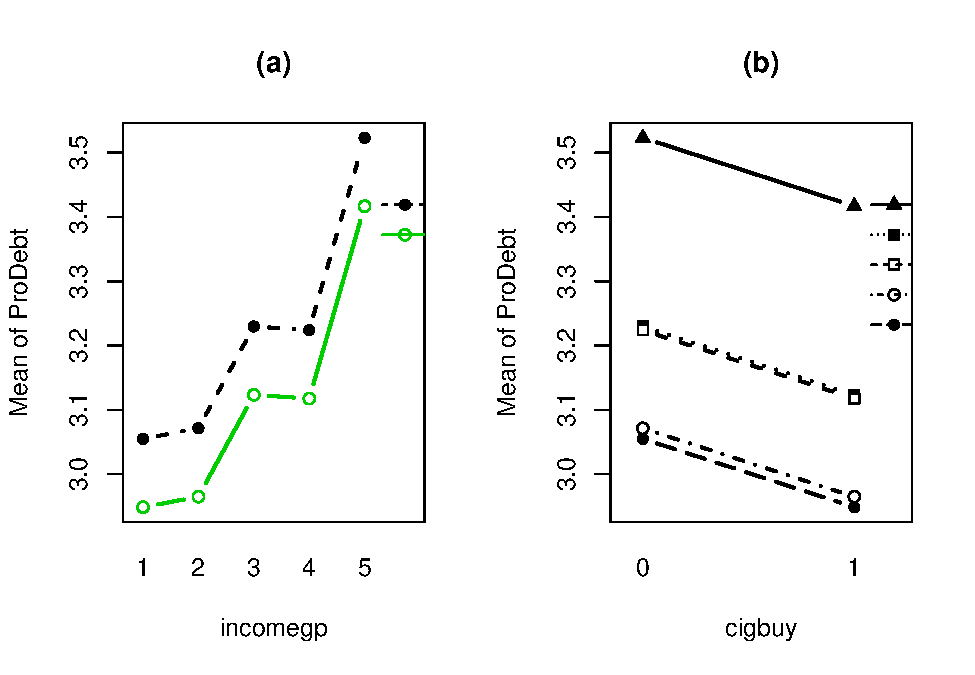
\includegraphics{04-twoWayAnova_files/figure-latex/Figure4-16-1.pdf}
\caption{\label{fig:Figure4-16}Illustration of the results from Table \ref{tab:Table4-2}
showing the combined impacts of the components of the additive model for
\texttt{prodebt}. Panel (a) uses income groups on the x-axis and
different lines for cigarette buyers (1) or not (0). Panel (b) displays
the different income groups as lines with the cigarette buying status on
the x-axis.}
\end{figure}

\textbf{In general, we proceed through the following steps in any 2-WAY
ANOVA situation:}

\begin{enumerate}
\def\labelenumi{\arabic{enumi}.}
\item
  Make an interaction plot.
\item
  Fit the interaction model; examine the test for the interaction.
\item
  Check the residual diagnostic plots for the interaction model
  (especially normality and equal variance).

  \begin{itemize}
  \tightlist
  \item
    If there is a problem with normality or equal variance, consider a
    ``transformation'' of the response as discussed in Chapter
    \ref{chapter7} This can help make the responses have similar
    variances or responses to be more normal, but sometimes not both.
  \end{itemize}
\end{enumerate}

\newpage

\begin{enumerate}
\def\labelenumi{\arabic{enumi}.}
\setcounter{enumi}{3}
\item
  If the interaction test has a small p-value, that is your main result.
  Focus on the interaction plot from (1) to fully understand the
  results, adding Tukey's HSD results to see which means of the
  combinations of levels are detected as being different.
\item
  If the interaction is not considered important, then re-fit the model
  without the interaction (additive model) and re-check the diagnostic
  plots. If the diagnostics are reasonable to proceed:

  \begin{itemize}
  \item
    Focus on the results for each explanatory variable, using Type II
    tests especially if the design is not balanced.
  \item
    Report the initial interaction test results and the results for the
    test for each variable from the model that is re-fit without the
    interaction.
  \item
    Model coefficients are interesting as they are shifts from baseline
    for each level of each variable, controlling for the other variable
    -- interpret those differences if the number of levels is not too
    great.
  \end{itemize}
\end{enumerate}

Whether you end up favoring an additive or interaction model, all steps
of the hypothesis testing protocol should be engaged.

\section{Pushing Two-Way ANOVA to the limit: Un-replicated
designs}\label{section4-6}

In some situations, it is too expensive to replicate combinations of
treatments and only one observation at each combination of the two
explanatory variables, A and B, is possible. In these situations, even
though we have information about all combinations of A and B, it is no
longer possible to test for an interaction. Our regular rules for
degrees of freedom show that we have nothing left for the error degrees
of freedom and so we have to drop the interaction and call that
potential interaction variability ``error''.

We can still perform an analysis of the responses but an issue occurs
with trying to estimate the interaction \(F\)-test statistic -- we run
out of degrees of freedom for the error. To illustrate these methods,
the paper towel example is revisited except that only one response for
each combination is used. Now the entire data set can be displayed:

\begin{Shaded}
\begin{Highlighting}[]
\NormalTok{ptR<-}\KeywordTok{read.csv}\NormalTok{(}\StringTok{"http://www.math.montana.edu/courses/s217/documents/ptR.csv"}\NormalTok{)}
\NormalTok{ptR}\OperatorTok{$}\NormalTok{dropsf<-}\KeywordTok{factor}\NormalTok{(ptR}\OperatorTok{$}\NormalTok{drops)}
\NormalTok{ptR}
\end{Highlighting}
\end{Shaded}

\begin{verbatim}
##   brand drops responses dropsf
## 1    B1    10 1.9064356     10
## 2    B2    10 3.0504173     10
## 3    B1    20 0.7737965     20
## 4    B2    20 2.8384124     20
## 5    B1    30 1.5557071     30
## 6    B2    30 0.5470565     30
\end{verbatim}

Upon first inspection the interaction plot in Figure
\ref{fig:Figure4-17} looks like there might be some interesting
interactions present. But remember now that there is only a single
observation at each combination of the brands and water levels so there
is not much power to detect differences in this sort of situation and no
replicates at combination that allow estimation of SEs so no bands are
produced in the plot.




\begin{figure}
\centering
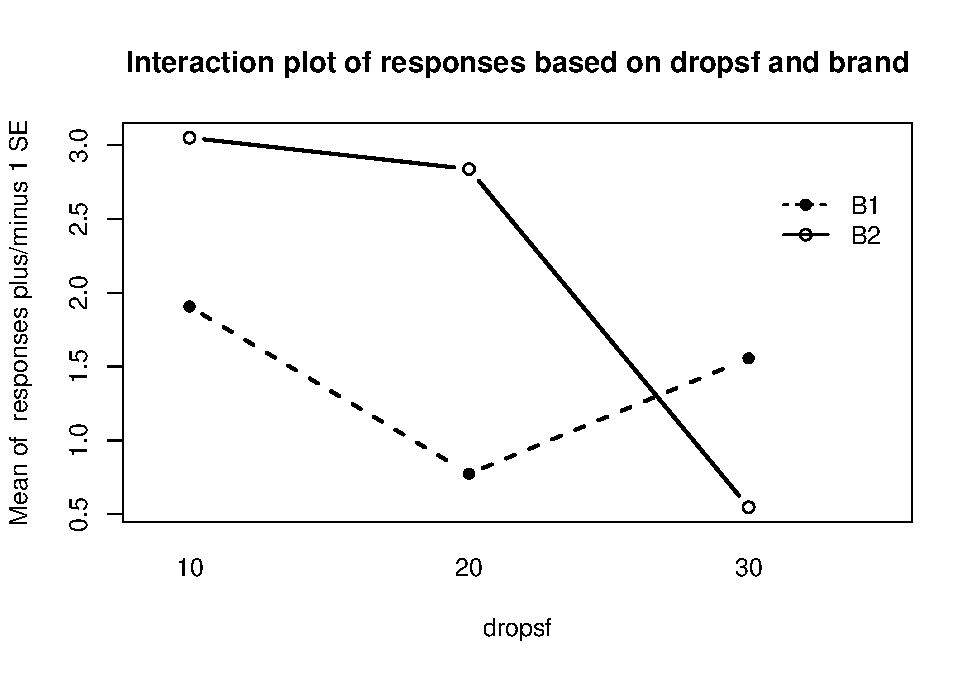
\includegraphics{04-twoWayAnova_files/figure-latex/Figure4-17-1.pdf}
\caption{\label{fig:Figure4-17}Interaction plot in paper towel data set with no
replication.}
\end{figure}

\begin{Shaded}
\begin{Highlighting}[]
\KeywordTok{par}\NormalTok{(}\DataTypeTok{mfrow=}\KeywordTok{c}\NormalTok{(}\DecValTok{1}\NormalTok{,}\DecValTok{1}\NormalTok{))}
\KeywordTok{intplot}\NormalTok{(responses}\OperatorTok{~}\NormalTok{brand}\OperatorTok{*}\NormalTok{dropsf,}\DataTypeTok{data=}\NormalTok{ptR,}\DataTypeTok{lwd=}\DecValTok{2}\NormalTok{)}
\end{Highlighting}
\end{Shaded}

The next step would be to assess the statistical evidence related to an
interaction between \texttt{Brand} and \texttt{Drops}. A problem will
arise in trying to form the ANOVA table as you would see this in the
console:

\small

\begin{verbatim}
> anova(lm(responses~dropsf*brand,data=ptR))
Analysis of Variance Table
Response: responses
             Df  Sum Sq Mean Sq F value Pr(>F)
dropsf        2 2.03872 1.01936               
brand         1 0.80663 0.80663               
dropsf:brand  2 2.48773 1.24386               
Residuals     0 0.00000                       
Warning message:
In anova.lm(lm(responses ~ dropsf * brand, data = ptR)) :
  ANOVA F-tests on an essentially perfect fit are unreliable
\end{verbatim}

\normalsize

Warning messages in R output show up in red after you run functions that
contain problems and are generally not a good thing, but can sometimes
be ignored. In this case, the warning message is not needed -- there are
no \(F\)-statistics or p-values in the results so we know there are some
issues with the results. The bolded line is key here squares of 0.
Without replication, there are no degrees of freedom left to estimate
the residual error. My (Greenwood's) first statistics professor, Gordon
Bril at Luther College, used to refer to this as ``shooting your load''
by fitting too many terms in the model given the number of observations
available. Maybe this is a bit graphic but hopefully will help you
remember the need for replication if you want to estimate interactions
-- it did for me. Without replication of observations, we run out of
information to estimate and test all the desired model components.

So what can we do if we can't afford replication? We can \emph{assume}
that the interaction does not exist and use those degrees of freedom and
variability as the error variability. When we drop the interaction from
Two-Way models, the interaction variability is added into the
\(\text{SS}_E\) so this is interaction between the variables. We are not
able to test for an interaction so must rely on the interaction plot to
assess whether an interaction might be present. Figure
\ref{fig:Figure4-17} suggests there might be an interaction in these
data (the two brands lines cross noticeably suggesting non-parallel
lines). So in this case, assuming no interaction is present is hard to
justify. But if we proceed under this dangerous assumption, tests for
the main effects can be developed.

\begin{Shaded}
\begin{Highlighting}[]
\NormalTok{norep1<-}\KeywordTok{lm}\NormalTok{(responses}\OperatorTok{~}\NormalTok{dropsf}\OperatorTok{+}\NormalTok{brand,}\DataTypeTok{data=}\NormalTok{ptR)}
\KeywordTok{Anova}\NormalTok{(norep1)}
\end{Highlighting}
\end{Shaded}

\begin{verbatim}
## Anova Table (Type II tests)
## 
## Response: responses
##            Sum Sq Df F value Pr(>F)
## dropsf    2.03872  2  0.8195 0.5496
## brand     0.80663  1  0.6485 0.5052
## Residuals 2.48773  2
\end{verbatim}

In the additive model, the last row of the ANOVA table that is called
the \texttt{Residuals} row is really the interaction row from the
interaction model ANOVA table. Neither main effect had a small p-value
(\texttt{Drops}: \(F(2,2)=0.82, \text{ p-value}=0.55\) and
\texttt{Brand}: \(F(1,2)=0.65, \text{ p-value}=0.51\)) in the additive
model. To get small p-values with small sample sizes, the differences
would need to be \textbf{very} large because the residual degrees of
freedom have become very small. The term-plots in Figure
\ref{fig:Figure4-18} show that the differences among the levels are
small relative to the residual variability as seen in the error bars
around each point estimate.




\begin{Shaded}
\begin{Highlighting}[]
\KeywordTok{plot}\NormalTok{(}\KeywordTok{allEffects}\NormalTok{(norep1))}
\end{Highlighting}
\end{Shaded}

\begin{figure}
\centering
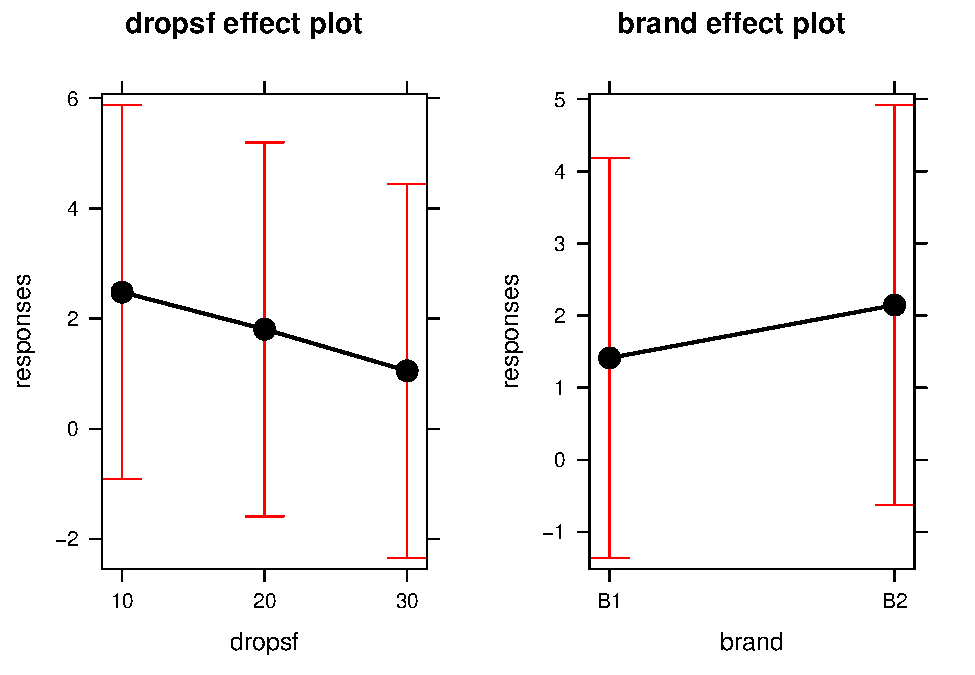
\includegraphics{04-twoWayAnova_files/figure-latex/Figure4-18-1.pdf}
\caption{\label{fig:Figure4-18}Term-plots for the additive model in paper towel data set
with no replication.}
\end{figure}

Hopefully by pushing the limits there are two conclusions available from
this section. First, replication is important, both in being able to
perform tests for interactions and for having enough power to detect
differences for the main effects. Second, dropping from the interaction
model to additive model, the variability explained by the interaction
term is pushed into the error term, whether replication is available or
not.

\section{Chapter summary}\label{section4-7}

In this chapter, methods for handling two different categorical
predictors in the same model with a continuous response were developed.
The methods build on techniques from Chapter \ref{chapter3} for the
One-Way ANOVA and there are connections between the two models. This was
most clearly seen in the guinea pig data set that was analyzed in both
chapters. When two factors are available, it is better to start with the
methods developed in this chapter because the interaction between the
factors can, potentially, be separated from their main effects. The
additive model is easier to interpret but should only be used when no
evidence of an interaction is present. When an interaction is determined
to be present, the main effects should not be interpreted and the
interaction plot in combination with Tukey's HSD provides information on
the important aspects of the results.

\begin{itemize}
\item
  If the interaction is retained in the model, there are two things you
  want to do with interpreting the interaction:

  \begin{enumerate}
  \def\labelenumi{\arabic{enumi}.}
  \item
    Describe the interaction, going through the changes from left to
    right in the interaction plot or term-plot for each level of the
    other variable.
  \item
    Suggest optimal combinations of the two variables to either get the
    highest or lowest possible responses.

    \begin{enumerate}
    \def\labelenumii{\alph{enumii}.}
    \tightlist
    \item
      For example, you might want to identify a dosage and delivery
      method for the guinea pigs to recommend and one to avoid if you
      want to optimize odontoblast growth.
    \end{enumerate}
  \end{enumerate}
\item
  If there is no interaction, then the additive model provides
  information on each of the variables and the differences across levels
  of each variable are the same regardless of the levels of the other
  variable.

  \begin{itemize}
  \tightlist
  \item
    You can describe the deviations from baseline as in Chapter
    \ref{chapter3}, but for each variable, noting that you are
    controlling for the variable.
  \end{itemize}
\end{itemize}

Some statisticians might have different recommendations for dealing with
interactions and main effects, especially in the context of evidence of
an interaction. We have chosen to focus on tests for interactions to
screen for ``real'' interactions and then interpret the interaction
plots aided by the Tukey's HSD for determining which combinations of
levels are detectably different. Others might suggest exploring the main
effects tests even with interactions present. In some cases, those
results are interesting but in others the results can be misleading and
wanted to avoid trying to tell you when that might happen. Consider two
scenarios, one where the main effects have large p-values but the
interaction has a small p-value and the other where the main effects and
the interaction all have small p-values. The methods discussed in this
chapter allow us to effectively arrive at the interpretation of the
differences in the results across the combinations of the treatments due
to the interaction having a small p-value. The main effects results are
secondary results at best when the interaction is important because we
know that impacts of one explanatory variable is changing based on the
levels of the other variable.

Chapter \ref{chapter5} presents a bit of a different set of statistical
methods that allow analyses of data sets similar to those considered in
the last two chapters but with a categorical response variable. The
methods are very different but are quite similar in overall goals to
those in Chapter \ref{chapter3} where differences in responses where
explored across groups. After Chapter \ref{chapter5}, the rest of the
semester will return to fitting models using the \texttt{lm} function as
used here, but incorporating quantitative predictor variables and then
eventually incorporating both categorical and quantitative predictor
variables. The methods in Chapter \ref{chapter8} are actually quite
similar to those considered here.

\section{Important R code}\label{section4-8}

The main components of R code used in this chapter follow with
components to modify in red, remembering that any R packages mentioned
need to be installed and loaded for this code to have a chance of
working:

\begin{itemize}
\item
  tally(\textcolor{red}{A}\textasciitilde{}\textcolor{red}{B},
  data=\textcolor{red}{DATASETNAME})

  \begin{itemize}
  \item
    Requires the \texttt{mosaic} package be loaded.
  \item
    Provides the counts of observations in each combination of
    categorical predictor variables A and B, used to check for balance
    and understand sample sizes in each combination.
  \end{itemize}
\item
  \textcolor{red}{DATASETNAME}\$\textcolor{red}{VARIABLENAME}
  \texttt{\textless{}-}
  factor(\textcolor{red}{DATASETNAME}\$\textcolor{red}{VARIABLENAME})

  \begin{itemize}
  \tightlist
  \item
    Use the \texttt{factor} function on any numerically coded
    explanatory variable where the numerical codes represent levels of a
    categorical variable.
  \end{itemize}
\item
  intplot(\textcolor{red}{Y}\textasciitilde{}\textcolor{red}{A}*\textcolor{red}{B},
  data=\textcolor{red}{DATASETNAME})

  \begin{itemize}
  \item
    Download and install using:
  \item
    \texttt{source("http://www.math.montana.edu/courses/s217/documents/intplot.R")}
  \item
    Provides interaction plot.
  \end{itemize}
\item
  \textcolor{red}{INTERACTIONMODELNAME} \texttt{\textless{}-}
  lm(\textcolor{red}{Y}\textasciitilde{}\textcolor{red}{A}*\textcolor{red}{B},
  data=\textcolor{red}{DATASETNAME})

  \begin{itemize}
  \item
    Fits the interaction model with main effects for A and B and an
    interaction between them.
  \item
    This is the first model that should be fit in Two-Way ANOVA modeling
    situations.
  \end{itemize}
\item
  \textcolor{red}{ADDITIVEMODELNAME} \texttt{\textless{}-}
  lm(\textcolor{red}{Y}\textasciitilde{}\textcolor{red}{A}+\textcolor{red}{B},
  data=\textcolor{red}{DATASETNAME})

  \begin{itemize}
  \item
    Fits the additive model with only main effects for A and B but no
    interaction between them.
  \item
    Should only be used if the interaction has been decided to be
    unimportant using a test for the interaction.
  \end{itemize}
\item
  summary(\textcolor{red}{MODELNAME})

  \begin{itemize}
  \tightlist
  \item
    Generates model summary information including the estimated model
    coefficients, SEs, t-tests, and p-values.
  \end{itemize}
\item
  Anova(\textcolor{red}{MODELNAME})

  \begin{itemize}
  \item
    Requires the \texttt{car} package to be loaded.
  \item
    Generates a Type II Sums of Squares ANOVA table that is useful for
    both additive and interaction models, but it most important to use
    when working with the additive model as it provides inferences for
    each term conditional on the other one.
  \end{itemize}
\item
  par(mfrow=c(2,2)); plot(\textcolor{red}{MODELNAME})

  \begin{itemize}
  \tightlist
  \item
    Generates four diagnostic plots including the Residuals vs Fitted
    and Normal Q-Q plot.
  \end{itemize}
\item
  plot(allEffects(\textcolor{red}{MODELNAME}))

  \begin{itemize}
  \item
    Requires the \texttt{effects} package be loaded.
  \item
    Plots the results from the estimated model.
  \end{itemize}
\end{itemize}

\newpage

\section{Practice problems}\label{section4-9}

To practice the Two-Way ANOVA, consider a data set on \(N=861\) ACT
Mathematics Usage Test scores from 1987. The test was given to a sample
of high school seniors who met one of three profiles of high school
mathematics course work: (a) Algebra I only; (b) two Algebra courses and
Geometry; and (c) two Algebra courses, Geometry, Trigonometry, Advanced
Mathematics, and Beginning Calculus. These data were generated from
summary statistics for one particular form of the test as reported by
\citet{Doolittle1989}. The source of this version of the data set is
\citet{Ramsey2012} and the \texttt{Sleuth2} package \citep{R-Sleuth2}.
First install and then load that package.

\begin{verbatim}
require(Sleuth2)
require(mosaic)
math <- ex1320
names(math)
favstats(Score ~ Sex+Background, data=math)
\end{verbatim}

4.1. Use the \texttt{favstats} summary to discuss whether the design was
balanced or not.

4.2. Make a side-by-side beanplot and interaction plot of the results
and discuss the relationship between Sex, Background, and ACT Score.

4.3. Write out the interaction model in terms of the Greek letters,
making sure to define all the terms and don't forget the error terms in
the model.

4.4. Fit the interaction plot and find the ANOVA table. For the test you
should consider first (the interaction), write out the hypotheses,
report the test statistic, p-value, distribution of the test statistic
under the null, and write a conclusion related to the results of this
test.

4.5. Re-fit the model as an additive model (why is this reasonable
here?) and use \texttt{Anova} to find the Type II sums of squares ANOVA.
Write out the hypothesis for the Background variable, report the test
statistic, p-value, distribution of the test statistic under the null,
and write a conclusion related to the results of this test.

4.6. Use the \texttt{effects} package to make a term-plot from the
additive model from 4.5 and discuss the results. Specifically, discuss
what you can conclude about the average relationship across both sexes,
between Background and average ACT score?

4.7. Make our standard diagnostic plots and assess the assumptions using
these plots. Can you assess independence using these plots? Discuss this
assumption in this situation.

4.8. Use the estimated model coefficients to determine which of the
combinations of levels provides the highest estimated average score.

\bibliography{packages,references}


\end{document}
